\chapter{System Architecture}
\label{c:system}
Two major components of our system are (a) processing of video frames using computer vision techniques to detect traffic lights and (b) selection of a subpart of a frame using inertial sensor hints to reduce both computation time and spurious detection of traffic lights. 
In this chapter, we present the end-to-end system and describe various components of the system pipeline.

%% In this chapter, we discuss the system overview for traffic light detection.
%% This system detects the color of a traffic light in a recorded video frame.
%% We captured video using a smartphone along with the sensor data.

\section{Overview}
\label{s:overview}

\begin{figure}
\centering
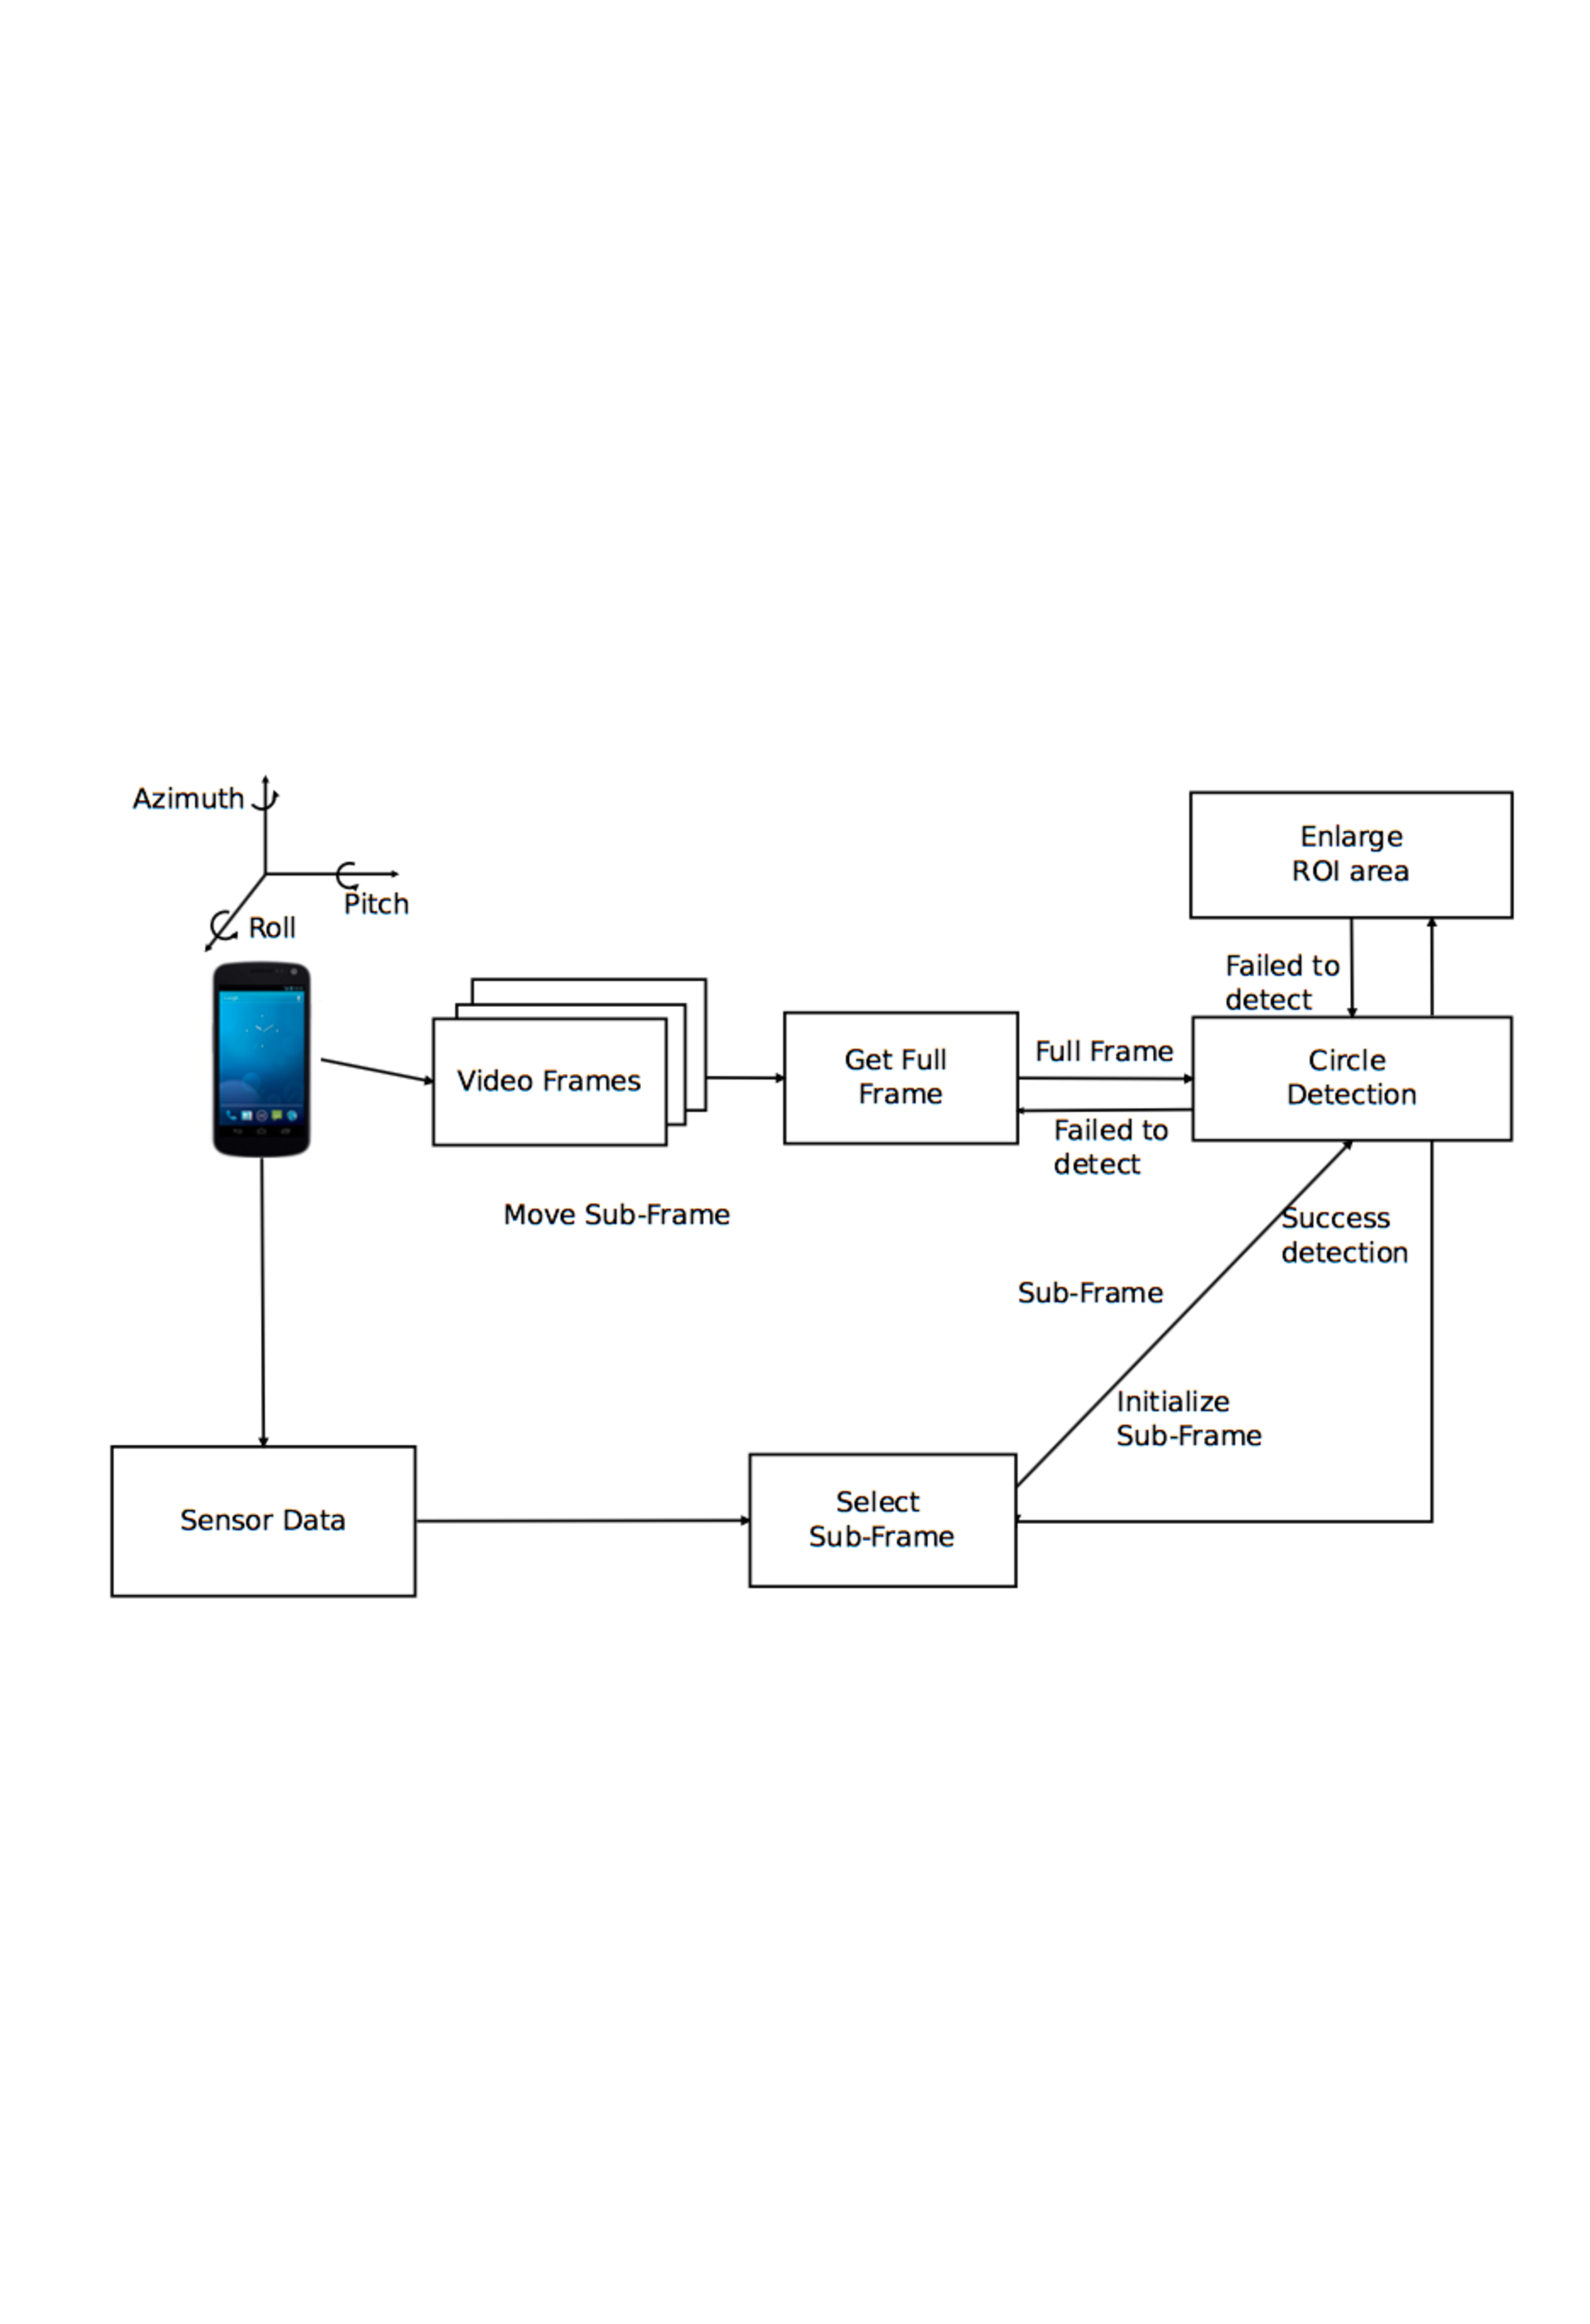
\includegraphics[width=5.2in]{figures/sysdia1.pdf}
\caption{System Overview}
\label{f:sys_dia}
\end{figure}

\ref{f:sys_dia} shows the overview of our system.
Using our smartphone app, we simultaneously record video and inertial sensor data.
Initially, we process the full region of the video frames to detect the traffic lights.
Once we successfully detect traffic lights in a video frame, we process only subparts of the subsequent frames using the sensor hints. 
For the subsequent frames, using the orientation change, we predict the region where the traffic lights are likely to move and process only that region for detecting the traffic lights.
However, the prediction of region-of-interest (ROI) using the sensor hints can sometimes be incorrect.
In such cases, we gradually increase the area of the ROI until we detect traffic lights in that enlarged area. 
Note that the increment of the ROI can go up to the whole frame if there are no traffic lights in the frame or the traffic light detection algorithm fails to detect the existing traffic lights. 

The algorithm to detect traffic lights is same irrespective of processing of the full frame or a subpart of the frame.
Below, we discuss the image processing algorithm for traffic light detection at first. 
Next, we discuss the procedure to select a subpart of a frame using sensor hints.


%We use three features of the traffic light, color, shape, and traffic bulb in a black box and the sensor feature of a smartphone as a system architecture for traffic light detection.
%% While recording the video we logged in the sensor data.
%% The first step of detection is the color filtering of the recorded videos.
%% Each video frames is consist of different colors.
%% In this step, each frame is filtered with only red and green pixel.
%% The traffic bulb shape is mostly circle.
%% To detect this characteristic we use Hough Circle  transformation\cite{hough_circle}.
%% Based on the traffic light detection position in video frames, we fix the region of interest area, which is a subpart of video frames.
%% After that, on next video frames the ROI change in respect to the sensor data. 


%% At first, we recorded videos along with the sensor data, gyroscope, accelerometer, pitch, roll, and azimuth.
%% These data have synchronization with our recorded video frames since we logged in sensor data while recording.
%% Now to detect the traffic light, we use three features of the traffic light.
%% Those are the color, shape of a traffic light and traffic light location in a black box.

\section{Image processing for traffic light detection}
The primary features of a traffic light are its bright red, yellow, or green color and the circular bulbs.
We use both these features for detecting the traffic lights. 
However, there can be other objects in the scene that can satisfy these properties such as circular red or green flower on people's clothing, red or green street signs etc.
To filter out such false detections, we use two heuristic filters, which utilize the fact that traffic lights are usually placed within a black box. 
Below, we discuss these procedures in detail.

%% The first step of detection algorithm is color filtering of video frames.
%% Color filtering step filters out these candidate pixels from the video frames.


\subsection{Color space conversion}
The first step in our image processing pipeline is color space conversion.
We convert the BGR color space to HSV space.
To detect a specific color in BGR space, we need to use three different components (B, G, R).
However, HSV space has the property that we can detect a color based the single component, hue.
The range of hue values of each color are well defined and we utilize this range to keep the pixels of the desired color.


\subsection{Color filtering}
After color space conversion, we select the pixels of a video frame that have either red or green color since these colors are the most distinctive features of traffic lights.
We detect the red or green color by their corresponding hue range in HSV space as discussed in \ref{s:color_space}. 
To find the exact range of hue for red and green colors of traffic lights, we analyzed the traffic lights' pixels to compute the hue value distribution.
Specifically, we computed the distribution of hue values of 200 frames that contain either red or green traffic lights. 

\ref{f:light_hue} shows the distribution of hue values for only the pixels that have a red or green traffic lights.
Based on this distribution, we selected the hue range for color filtering. 
These ranges are shown in \ref{t:hue_range}.


\begin{figure}[!ht]
\centering
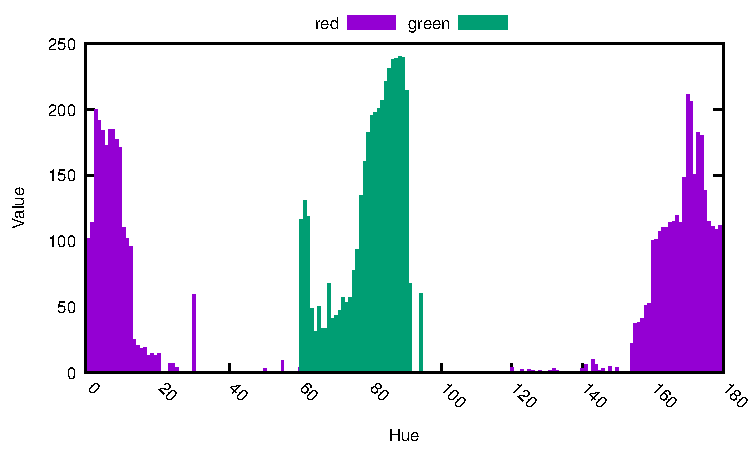
\includegraphics[width=5.2in]{plots/stat_light.pdf}
\caption{Statistics for hue range of green and red light.}
\label{f:light_hue}
\end{figure}


\begin{table}[h!]
  \centering
  \caption{Hue range for red and green pixel.}
  \label{t:hue_range}
  \begin{tabular}{  l | c  }
    \hline
    Hue range for red & Lower 0 to 10 \\ \cline{2-2}
    & Upper 160 to 179 \\
    \hline \hline
    Hue range for green & 65 to 95 \\
    \hline
  \end{tabular}
\end{table}


We only keep red and green pixels of a video frame for further processing in next stages.
Figure \ref{f:red} shows an example video frame with red traffic lights and figure \ref{f:green} shows an example video frame with green traffic lights.

\begin{figure*}[!ht]
\centering
\subfloat[Frame with red lights] {\label{f:red}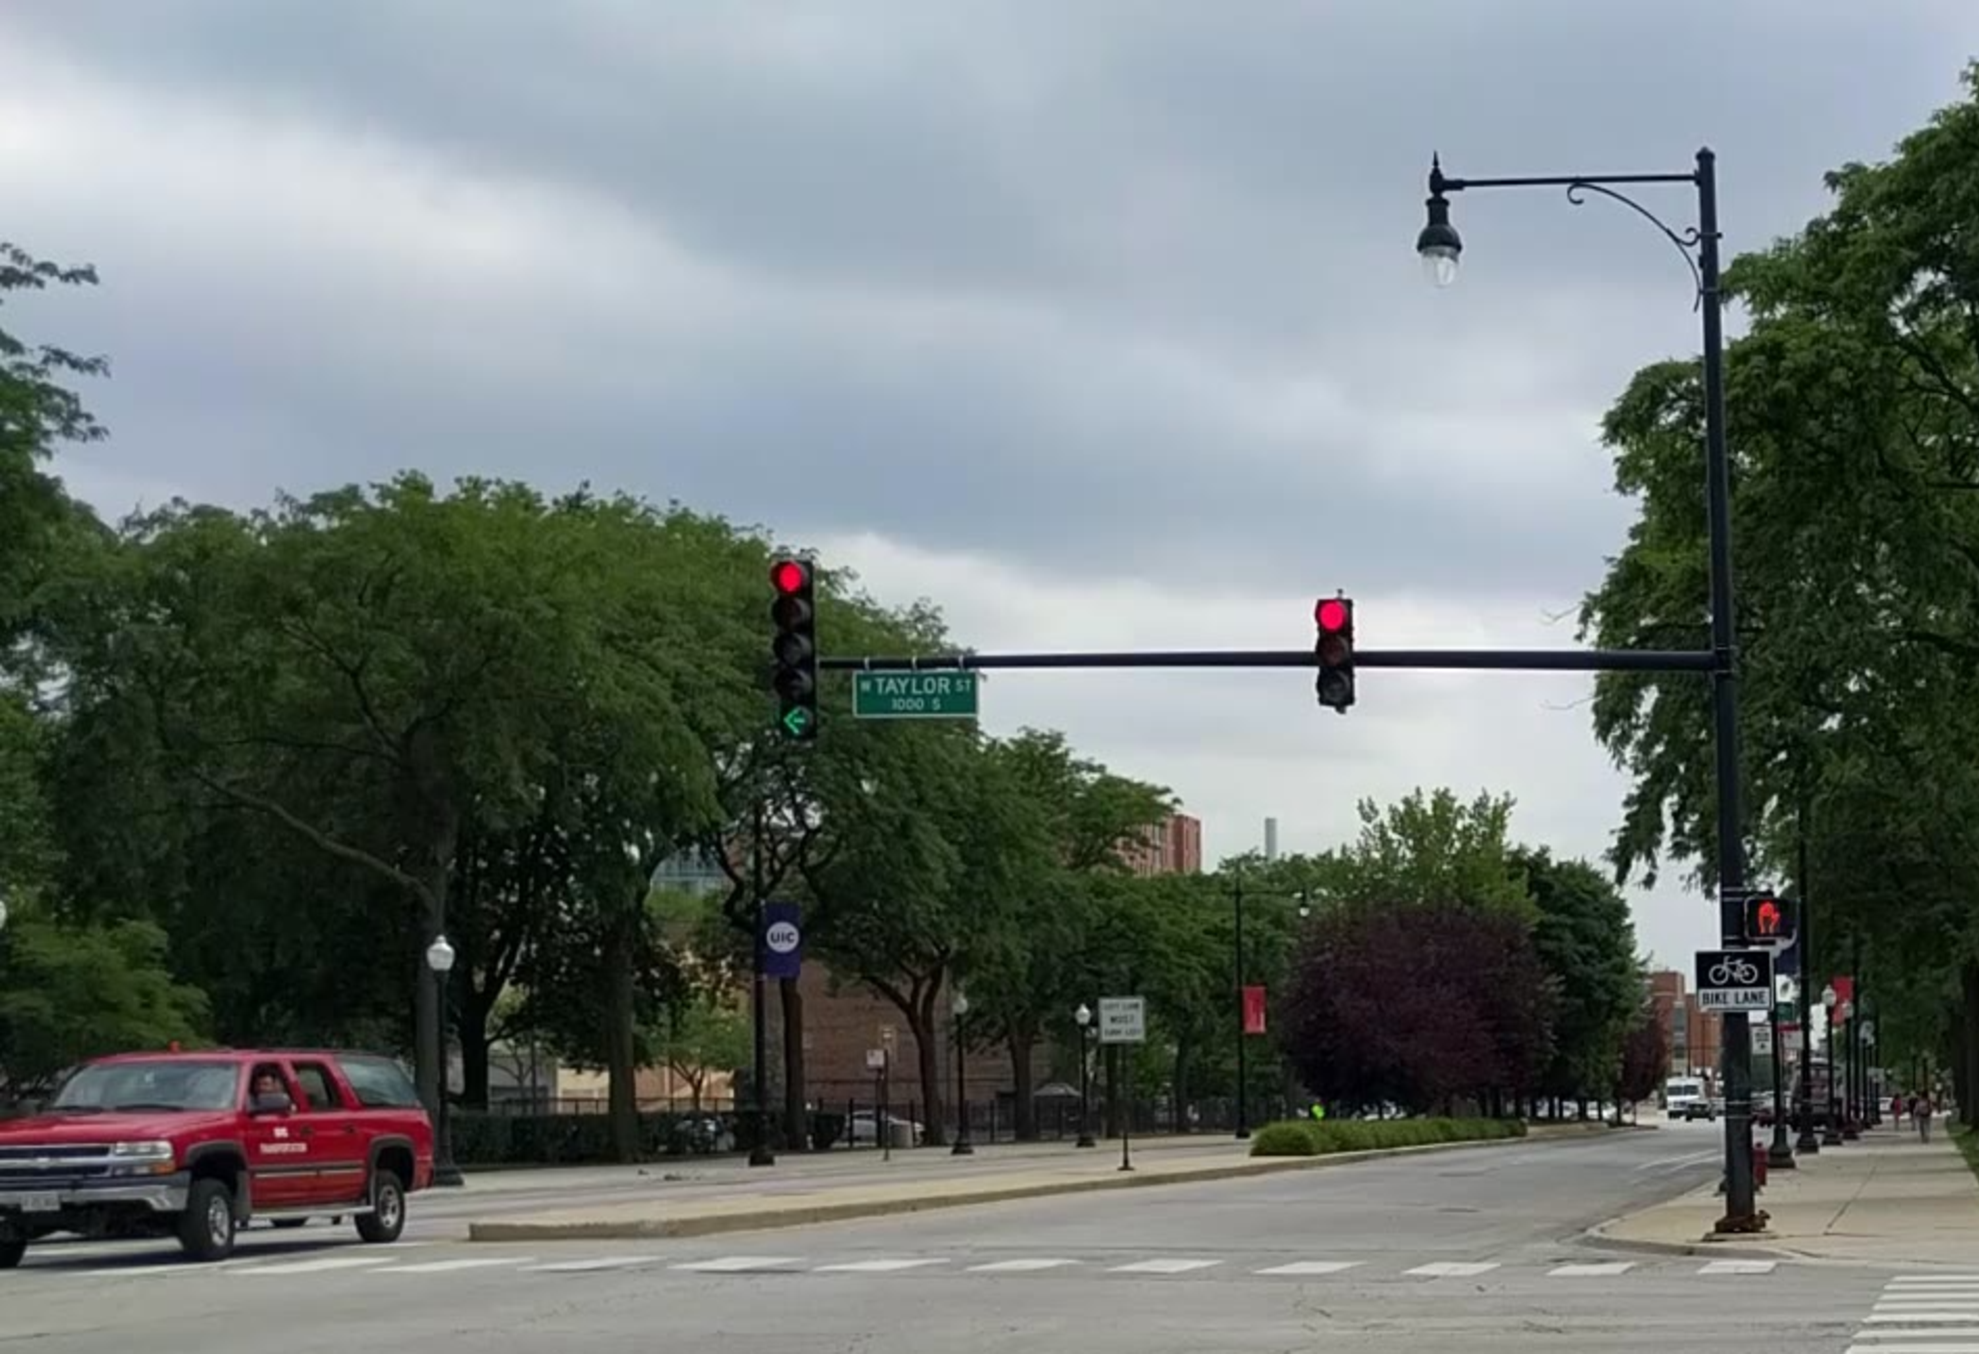
\includegraphics[width=3in]{images/frame301.pdf}}
\hfill
\subfloat[Frame with green lights] {\label{f:green}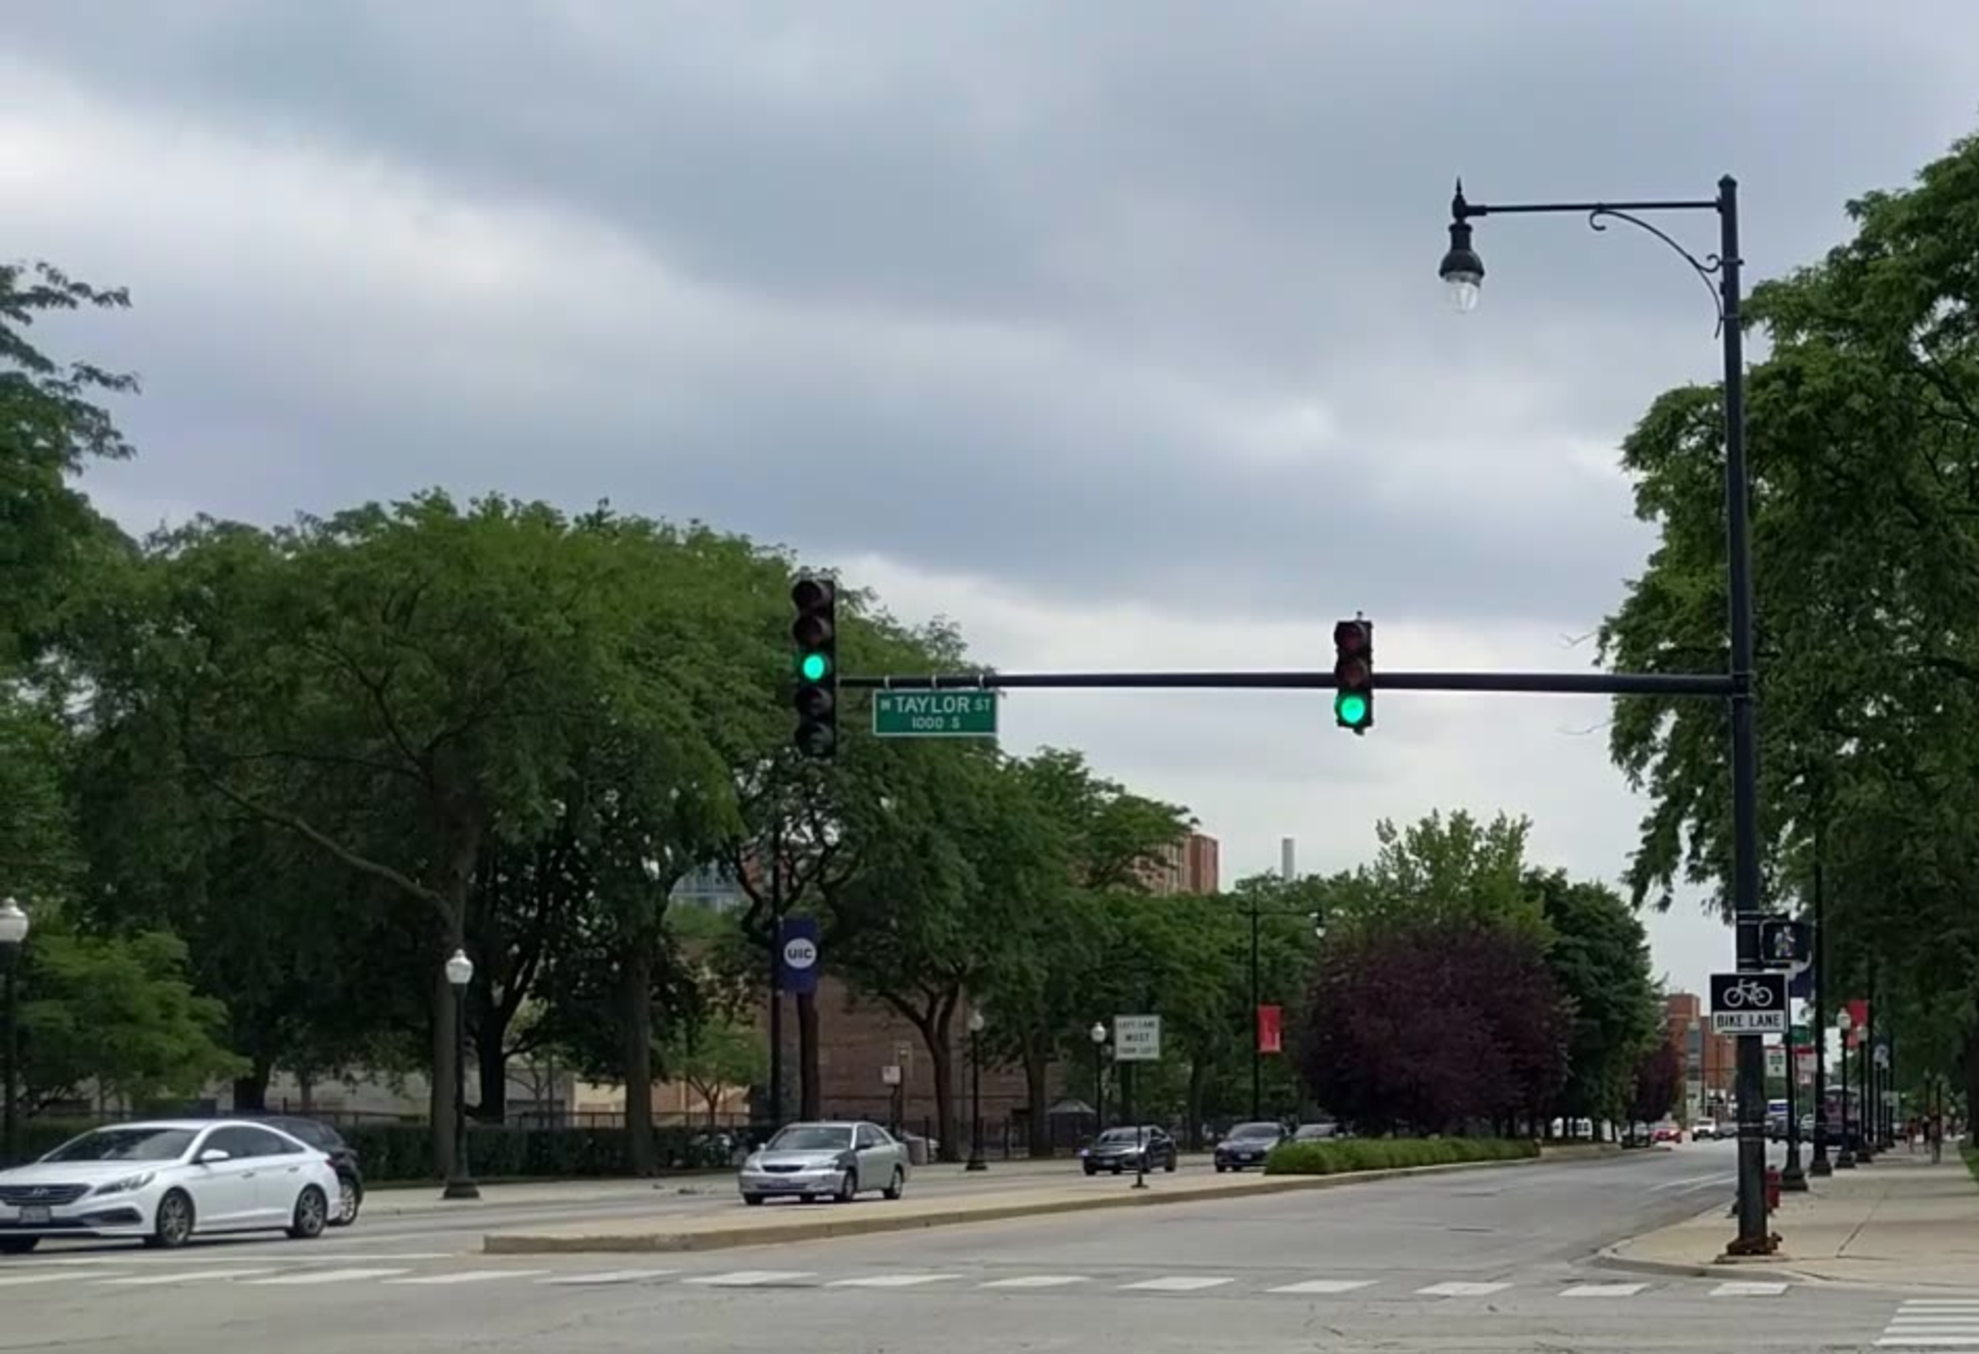
\includegraphics[width=3in]{images/frame502.pdf}}
\caption{Original video frames.}
\label{f:org_img}
\end{figure*}


\ref{f:fil_img} shows the frames after filtering out pixels except for the red and green color. 
\ref{f:fil_img} shows that the color filtering works well as it can isolate the traffic lights. 
However, there can be other objects with the red and green color in the scene such as a red car in \ref{f:red_fil} and a green road sign in both \ref{f:red_fil} and \ref{f:green_fil}.
We filter out such objects in next stages where we verify the circular shape of a traffic light and a black box around the light.
The color filtering process is computationally very lightweight.
Additionally, a significant benefit of this filtering process is that the computation time for the next stages is reduced by a large factor.
as the pixels with the zero value are not processed.


\begin{figure*}[!ht]
\centering
\subfloat[Frame with red lights] {\label{f:red_fil}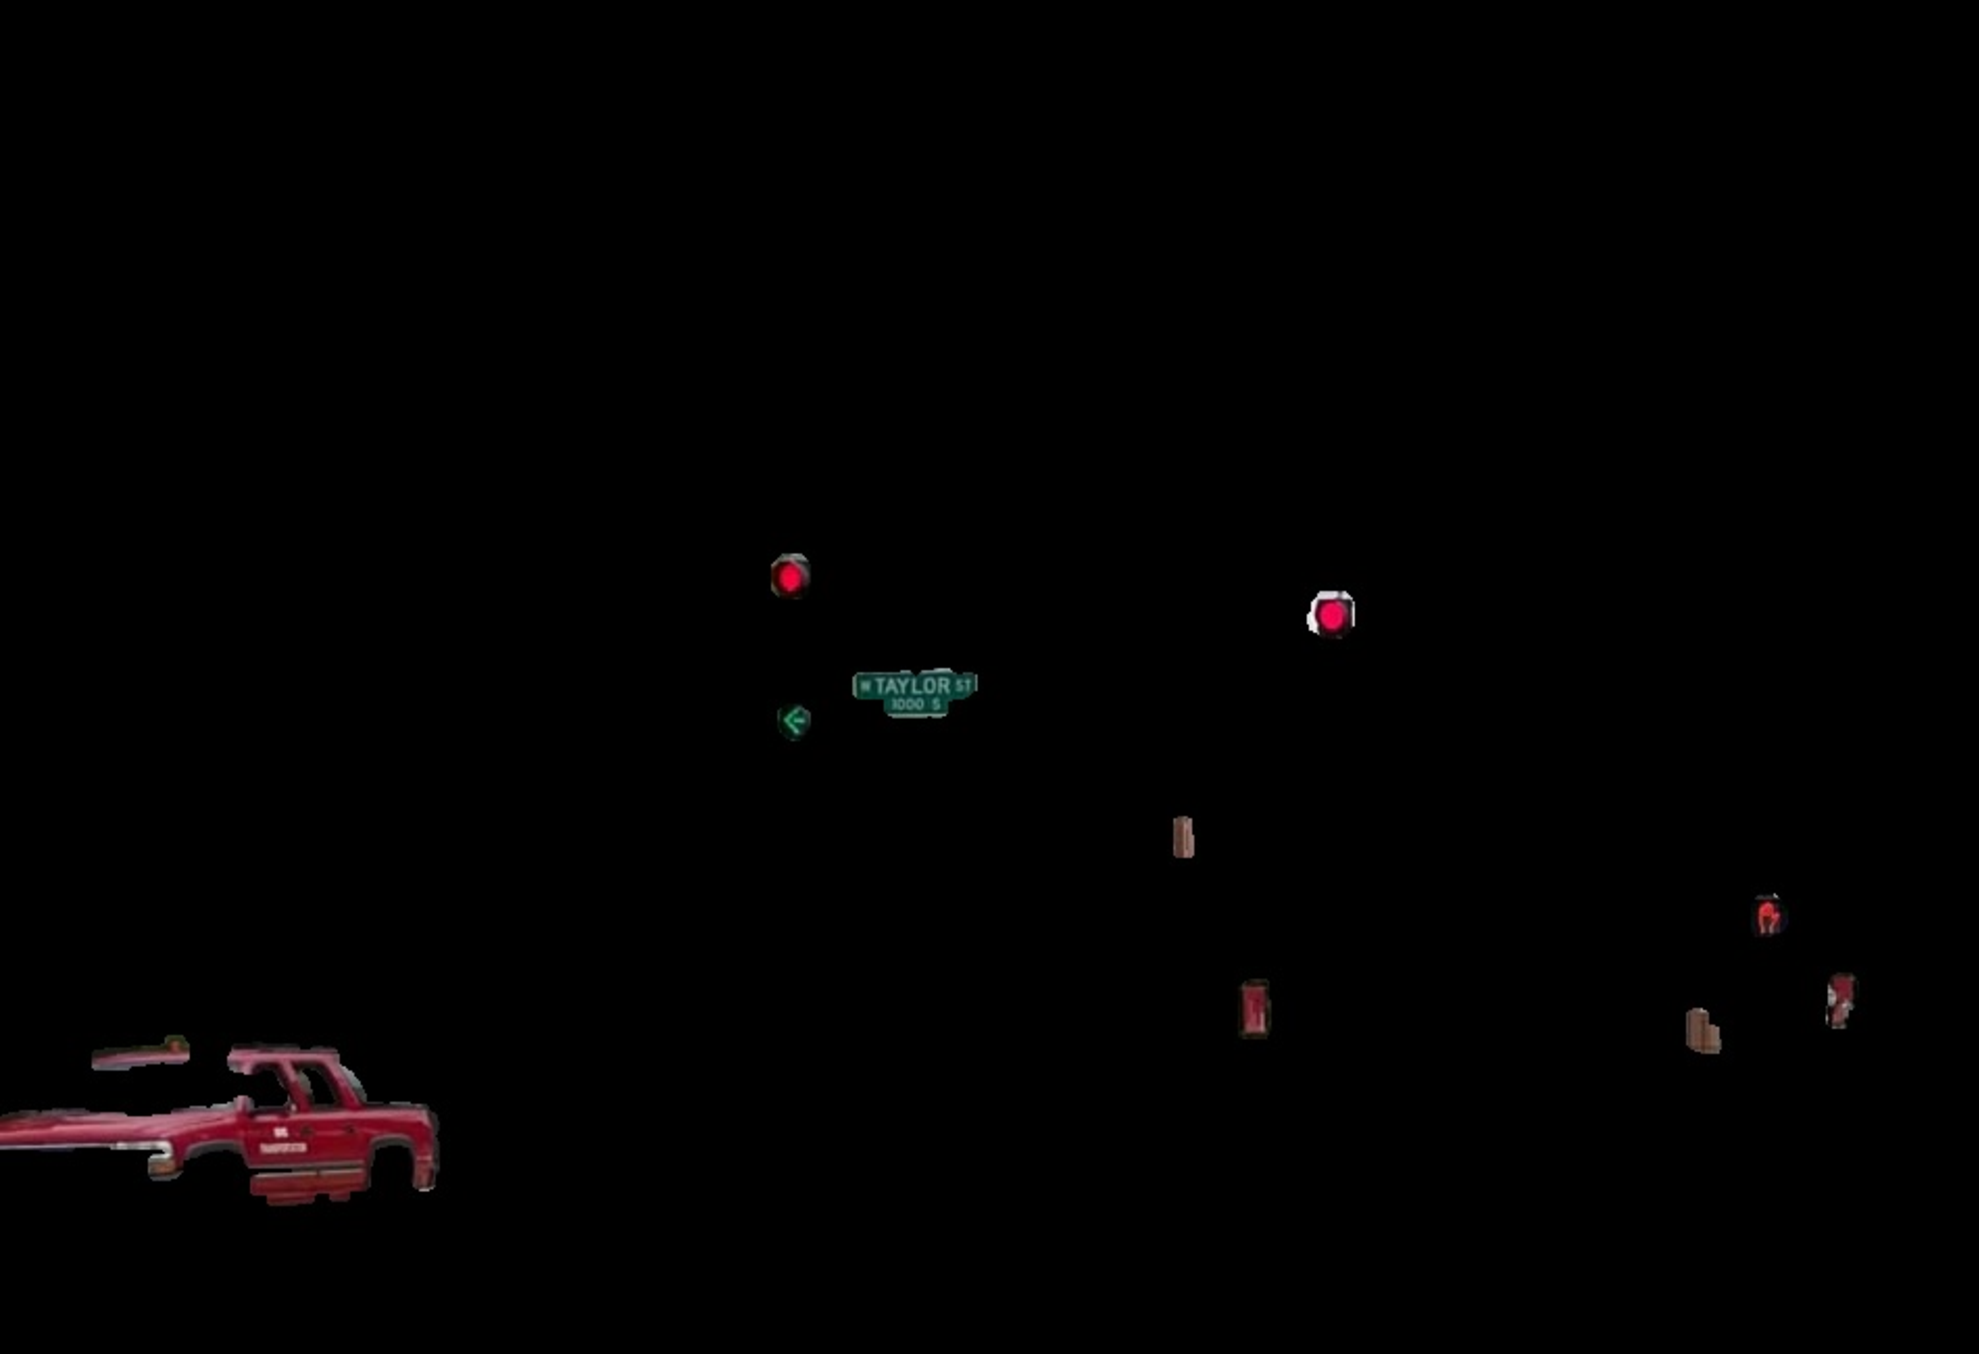
\includegraphics[width=3in]{images/RedGreenfiltering_red.pdf}}
\hfill
\subfloat[Frame with green lights] {\label{f:green_fil}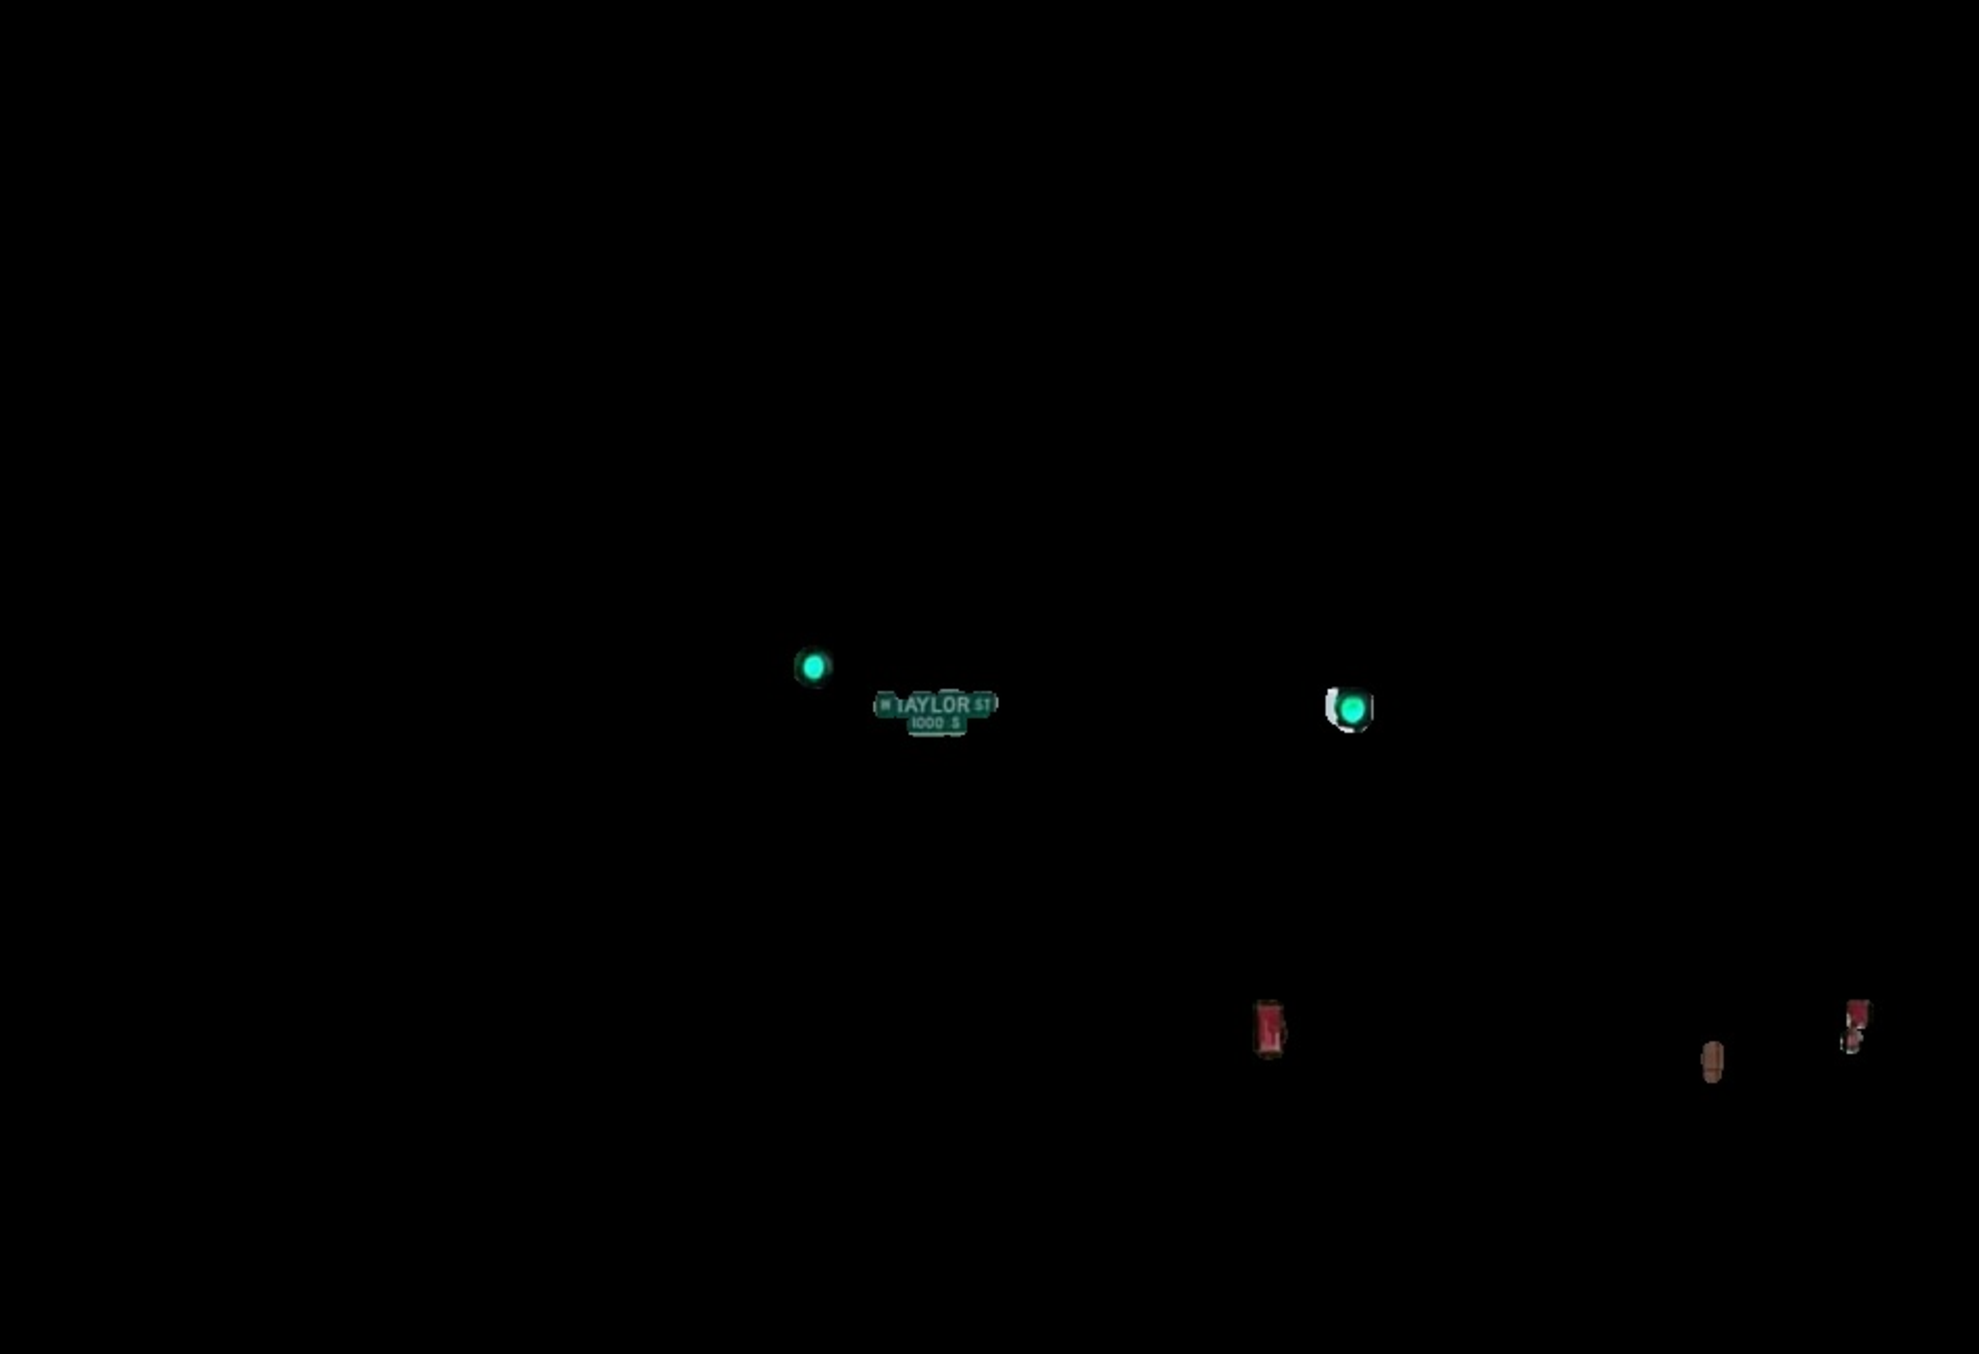
\includegraphics[width=3in]{images/RedGreenfiltering.pdf}}
\caption{Red green pixel filtering.}
\label{f:fil_img}
\end{figure*}


\ref{f:clrfil} shows the computation time of a video frame with and without the color filtering. 
Here, the median processing time reduces from 2000 ms to 67 ms approximately with color filtering, resulting in a speed up of 30x. 


\begin{figure}[h]
\centering
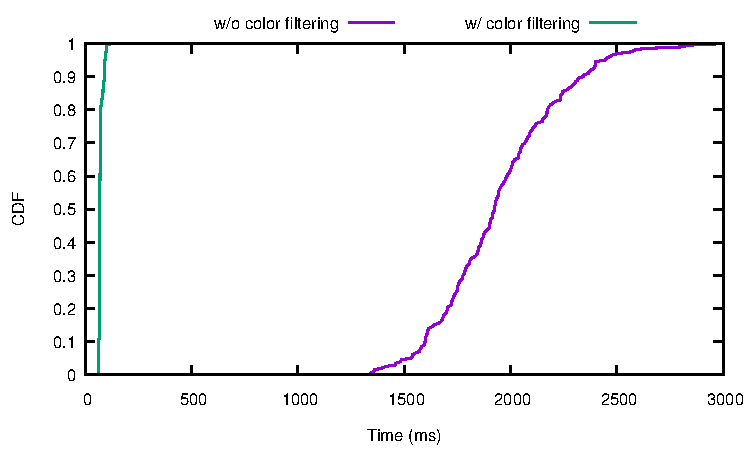
\includegraphics[width=5.2in]{plots/cdf_clrfil_full.pdf}
\caption{CDF for computational time comparison of the full video frames with and without color filtering technique.}
\label{f:clrfil}
\end{figure}


\subsection{Circularity check}
After color filtering, we detect the circular shape of the traffic light bulb to filter out other objects in the scene with red or green color (e.g., red car and green street sign in \ref{f:fil_img}).
Before Hough circle detection, we perform denoising and smoothing of a video frame with a median filter and Gaussian filter respectively so that circles are not detected due to noise and edged artifacts in the frame.
After the denoising and smoothing, we detect the circular traffic light bulbs using the Hough circle algorithm.

\ref{f:cir_img} shows example video frames after Hough circle detection.
Specifically, \ref{f:red_cir} shows the detected red traffic bulbs and \ref{f:green_cir} shows the detected green traffic bulbs.
Here, Hough circles detector successfully extracts the circular green and traffic light bulbs despite other red and green pixels in the video frames.


\begin{figure*}[!ht]
\centering
\subfloat[Frame with red lights] {\label{f:red_cir}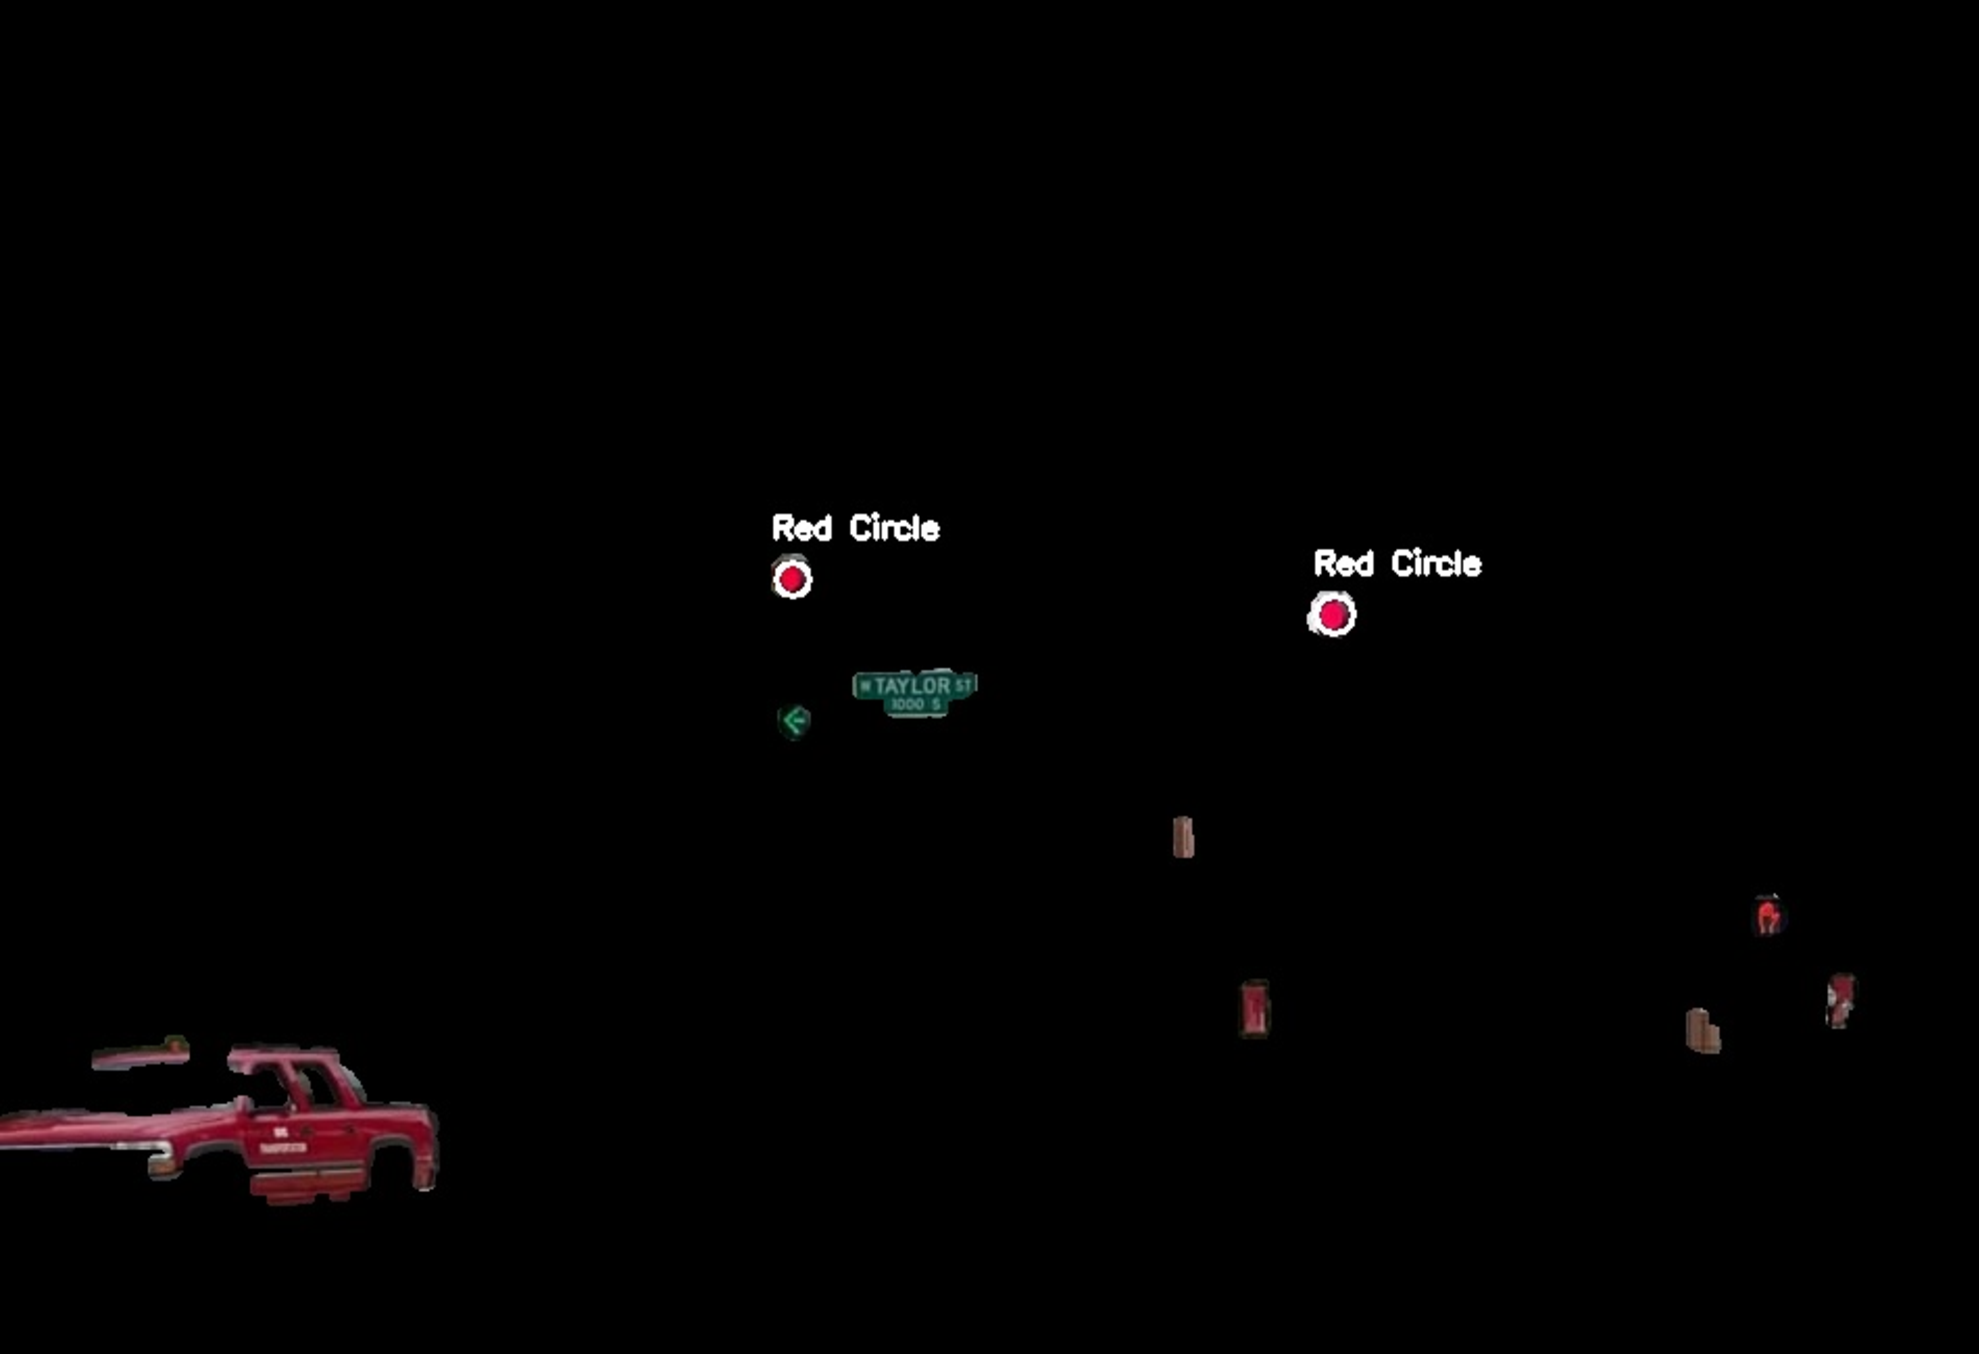
\includegraphics[width=3in]{images/Detectedredcircles.pdf}}
\hfill
\subfloat[Frame with green lights] {\label{f:green_cir}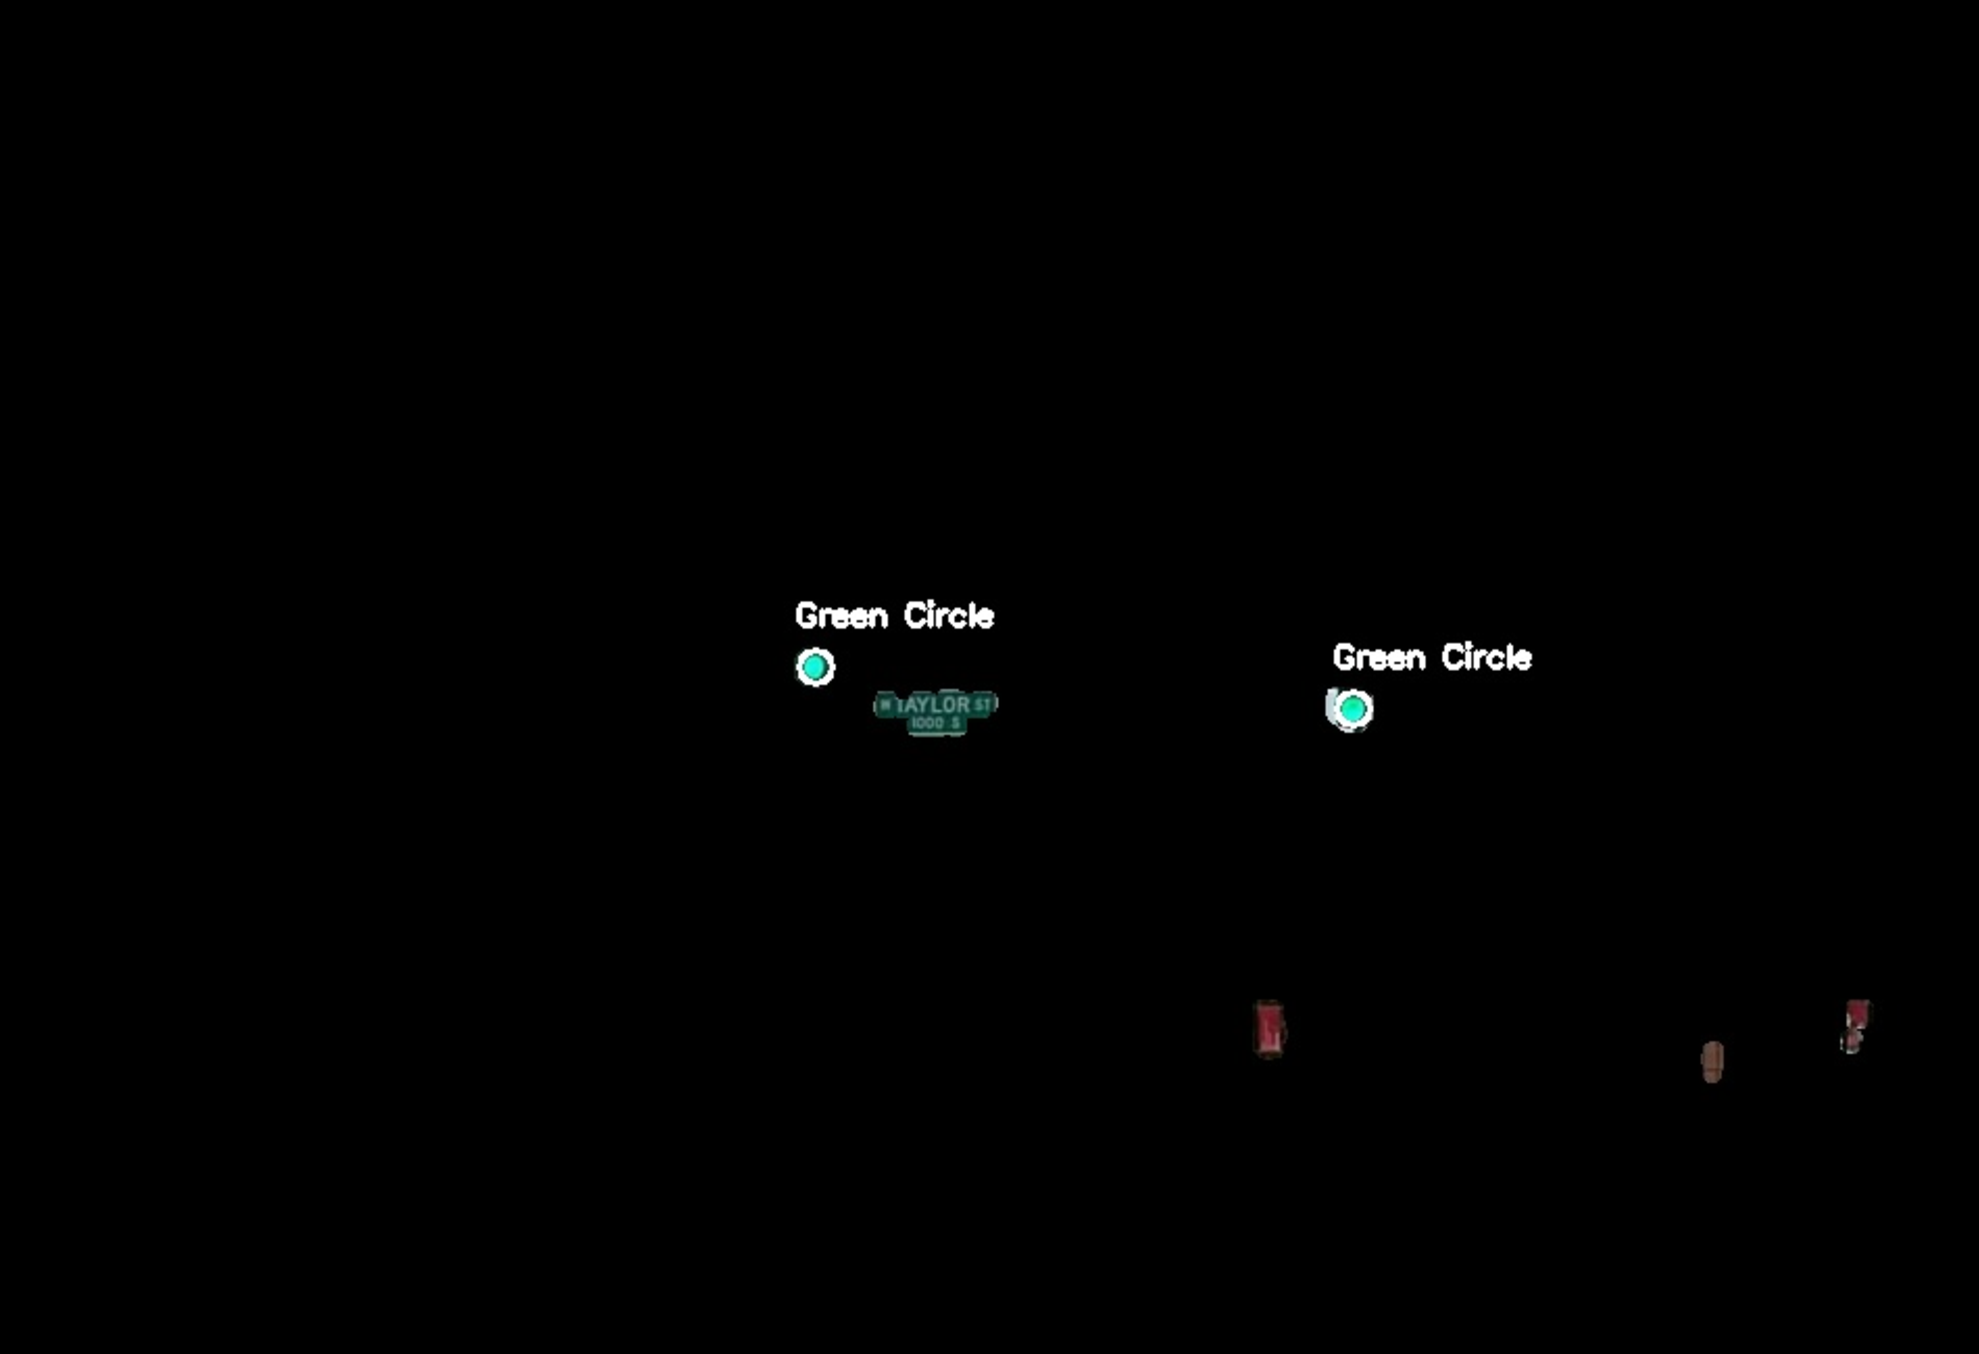
\includegraphics[width=3in]{images/Detectedgreencircles.pdf}}
\caption{Red green traffic bulb detection.}
\label{f:cir_img}
\end{figure*}


\subsection{Heuristic filters}
\label{s:filter}
At this point, we have the knowledge of the traffic bulb location and size (radius).
However, there can be still other objects in the scene that can have both green or red color and circular shape (e.g., flower on people's cloth).
In this final filtering stage, we attempt to remove such objects. 
Here, we take advantage of the fact that traffic light bulb resides inside a rectangular black box (see \ref{f:org_img}), and hence the pixels nearby the circular light bulb's perimeter should be black.
To check for this constraint, we experimented with two heuristics: (a) black mid-point circle verification \cite{midpoint}, (b) black rectangle box verification.

\subsubsection{Black mid-point circle verification}
In this heuristic, we check pixels intensity of a circular area outside but nearby of the traffic bulb.
We use midpoint circle algorithm to find the values of pixels on a circular perimeter which is larger than our traffic bulb size.
If at least 70\% of those pixel values are black then we consider it as a traffic light bulb.
We used the range from 0 to 45 in HSV color space as black.

While in principle this heuristic is sound, in our experiments the performance of this heuristic was not very good. 
The primary reason for the poor performance of this heuristic can be seen in \ref{f:bulb_int}.
Here, the red and green color is spread out a lot due to the high intensity of the traffic light bulbs. 
As a result, the pixels on the circle outside the perimeter mostly have red or green values instead of black.
Furthermore, we cannot check the pixels that are a lot further than the traffic bulb perimeter since the black box is not covered in that case.


\begin{figure*}[ht]
\centering
\subfloat[Red traffic bulb] {\label{f:red_bulb}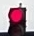
\includegraphics[width=2.2in]{images/redlight.jpg}}
\hfill
\subfloat[Green traffic bulb] {\label{f:green_bulb}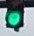
\includegraphics[width=2.2in]{images/greenlight.jpg}}\\

\caption{Red and green traffic bulb intensity.}
\label{f:bulb_int}
\end{figure*}


\subsubsection{Black rectangle verification}
In this heuristic, we check for a black square with the side equal to the diameter of the circular traffic light bulb.
Generally, traffic bulbs are located in a rectangular black square that can either horizontal or vertical.
Hence, we check the pixel values in four squares around a traffic bulb and we consider the traffic light to be correctly detected if one of these boxes is black.
We classify a square as black if at least 70\% of the pixels in that square are black.
We used the range from 0 to 45 in HSV color space as black.

\ref{f:norec_filter} shows that there is a false positive for green between two red traffic lights without the black rectangle heuristic.
This is a traffic sign and not a traffic light.
Once we apply the heuristic filter, this false detection is removed as shown in \ref{f:rec_filter}.

\begin{figure}[!ht]
\centering
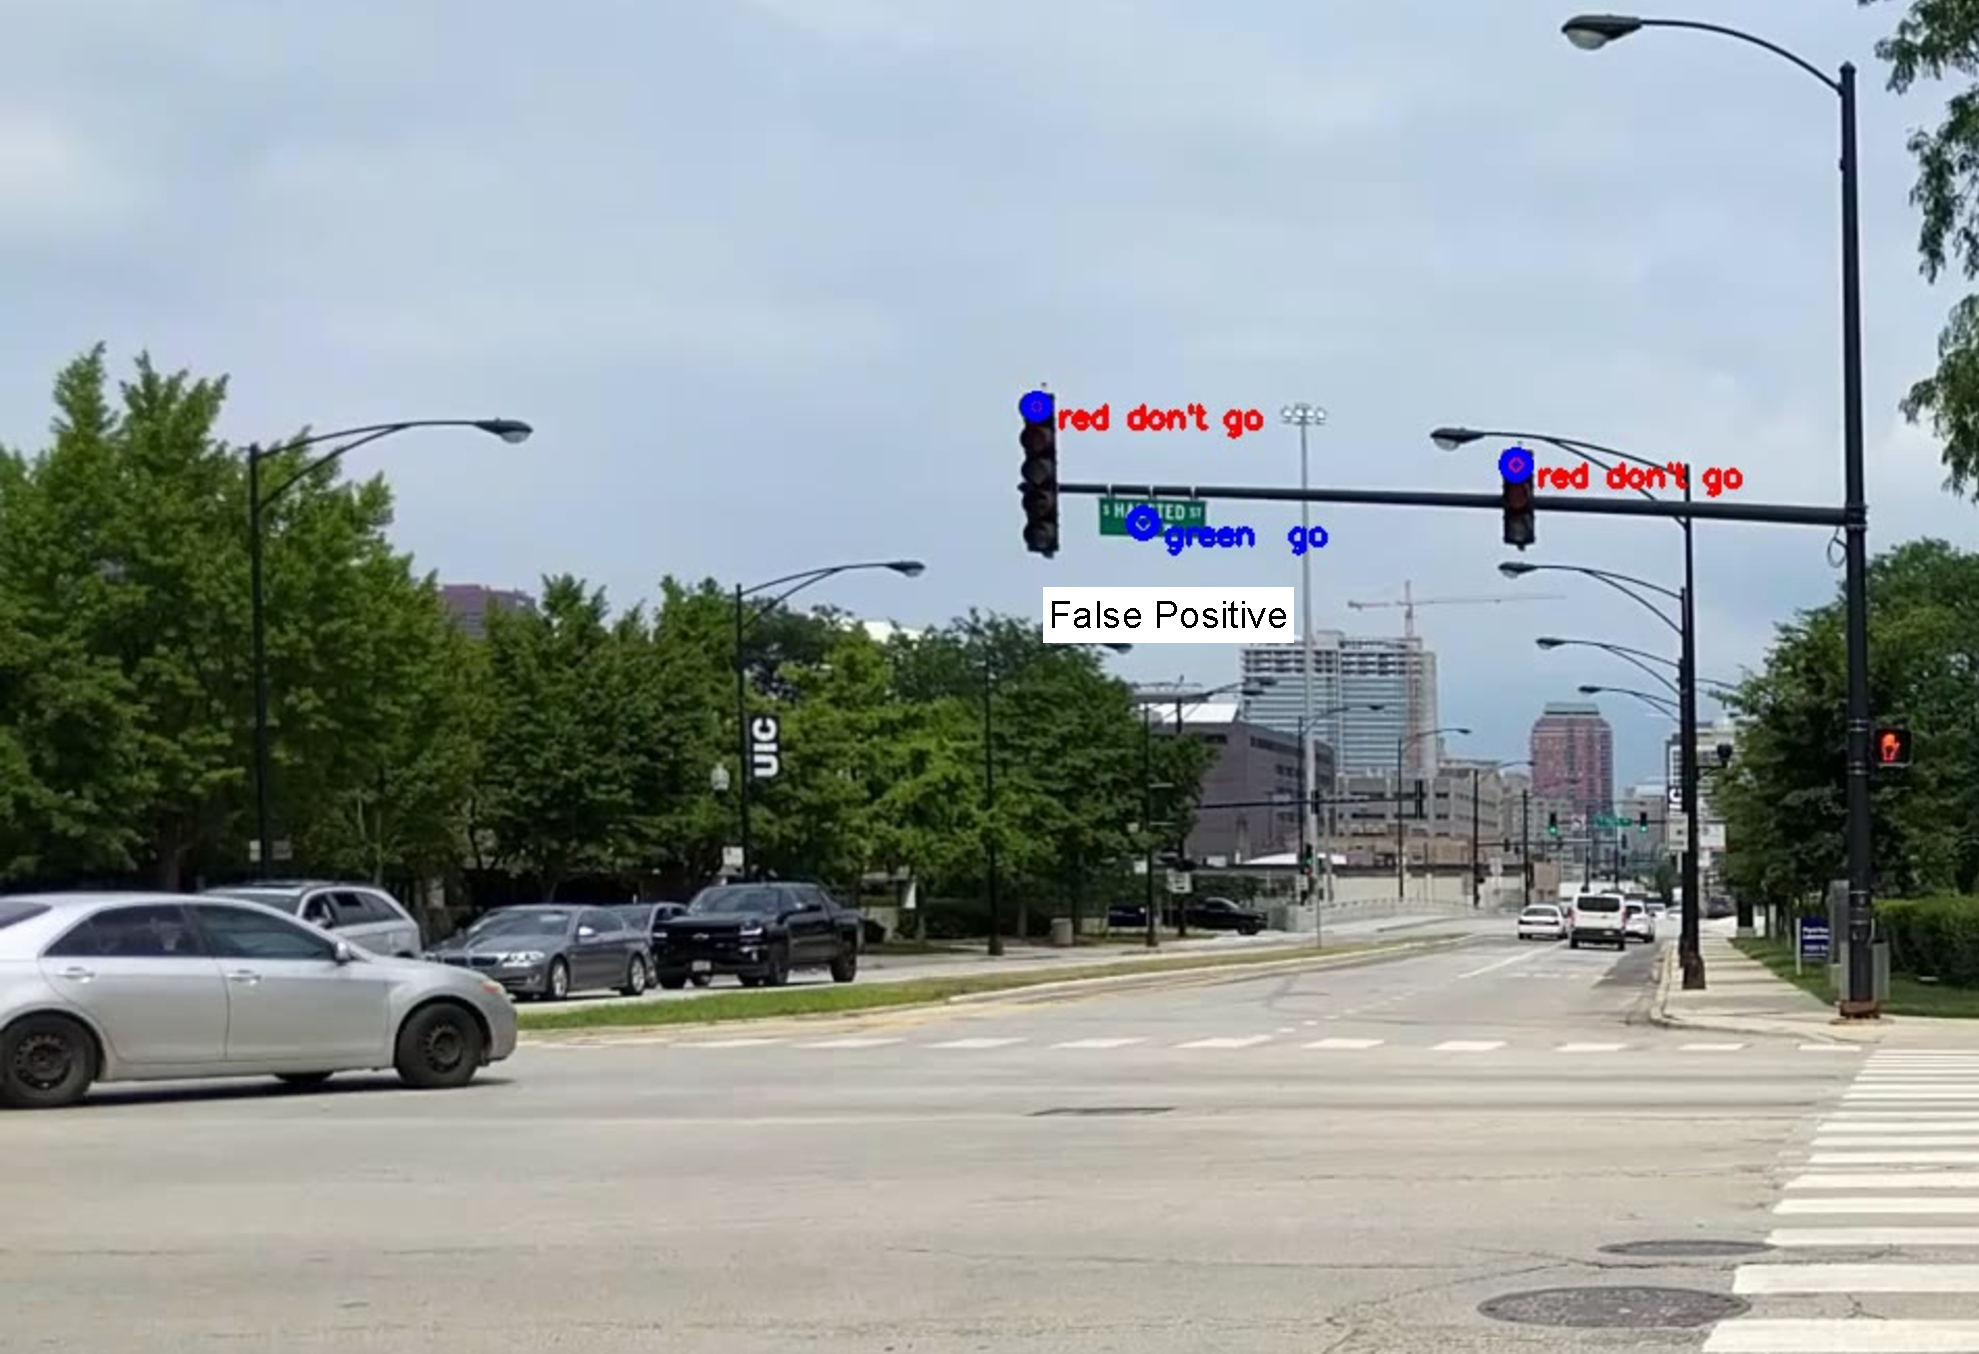
\includegraphics[width=4.2in]{images/norec_filter.pdf}
\caption{Output not using black box checking filter.}
\label{f:norec_filter}
\end{figure}



\begin{figure}[ht!]
\centering
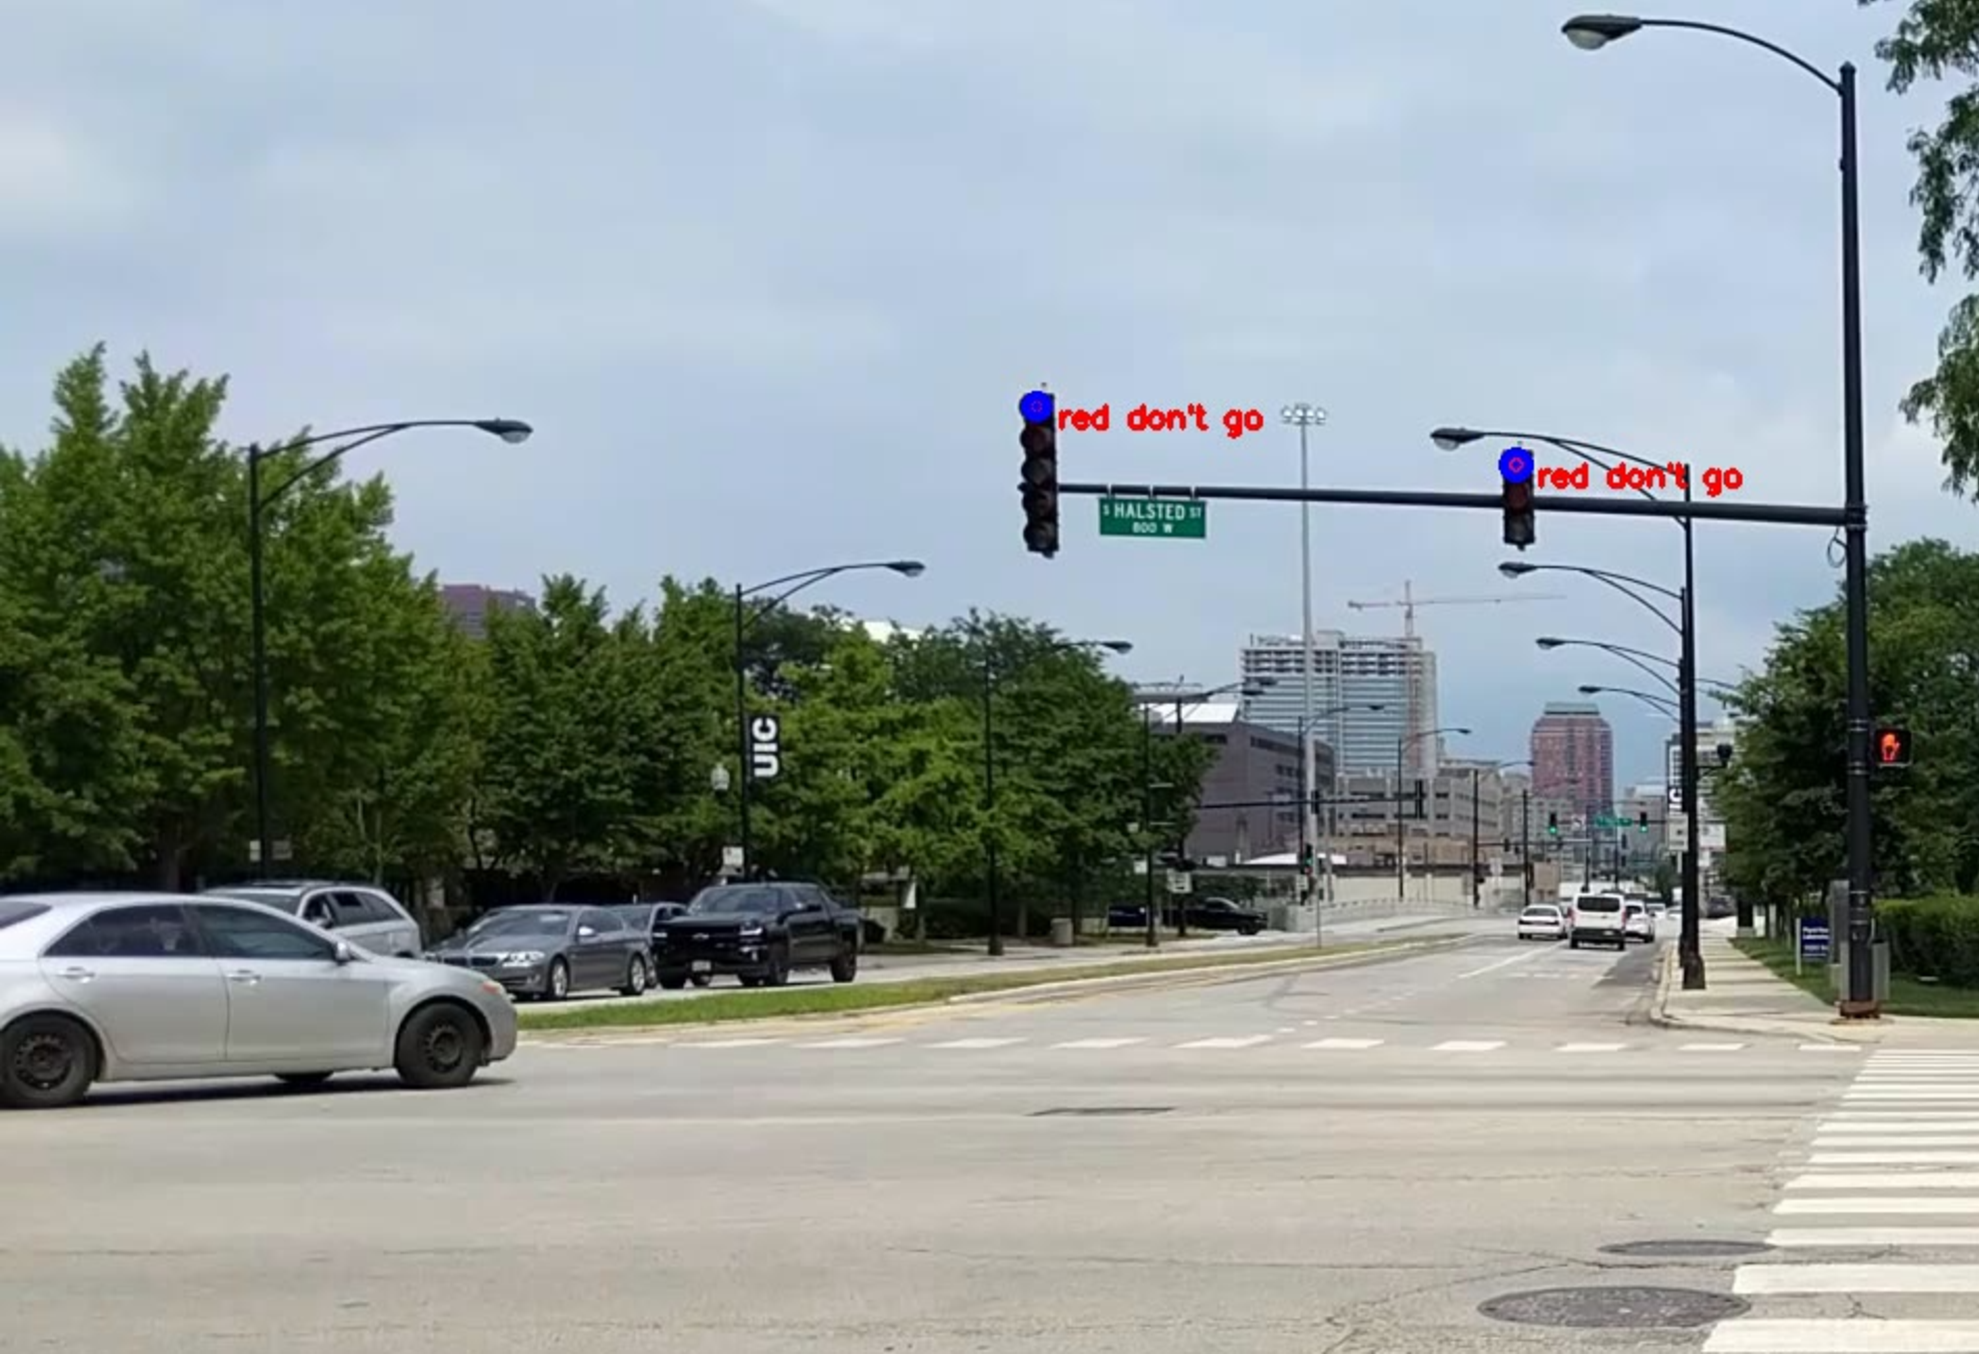
\includegraphics[width=4.2in]{images/rec_filter.pdf}
\caption{Output using black box checking filter.}
\label{f:rec_filter}
\end{figure}




\section{Sensor fusion for frame subpart selection}
Motion and orientation estimation of a smartphone with sensor fusion provide a big opportunity for processing a subpart of video frame instead of the whole frame for traffic light detection, resulting in an improvement in both computation time and accuracy.
In this section, we discuss about our sensor fusion algorithm. 

\subsection{Synchronization of sensors and video frames}
To improve traffic light detection we use the smartphone's sensor data.
We logged the sensor data simultaneously while recording the video.
The sensor data rate is lower than the frame rate. 
Specifically, we recorded the video at 30 frames per seconds and sensor data at 5 times per seconds. 
We synchronize the video frames with the sensor data according to the closest timestamp.
For intermediate video frames, we simply interpolate the sensor data.

%% From the logged data we know the time for sensor data registered.
%% We have the time when the video is recorded.
%% After that, we synchronized our data with the video using the starting time of the video and the frame rate.
%% So, using the frame rate and starting time we know the time for each frame, and from the logged sensor data, we know the sensor value corresponds to the time.
%% Using this time and our frame time we interpolated sensor hints if we miss any data corresponding to that frame.
%% Finally, we get the synchronized sensor data with our recorded video.

%\ref{} shows the interface of our android app.
%So when we start recording the pitch, roll and azimuth display in the screen and also start registering in a file.

\subsection{Region-Of-Interest selection}
\label{s:roi}
At first, we detect traffic lights in the video frames using the color, circular shape, and position of the traffic light bulbs inside a black box.
Once we have the initial position fix of the traffic lights in a video, we can utilize the orientation computed from the sensor hints to process only a subpart of the subsequent video frames. 
%With this idea we subdivide our video frame making a region of interest area.
As we move to the subsequent frames, we use the pitch, roll, and azimuth obtained from sensor fusion to predict the new ROI.
Using these sensor data of the current frame and the previous frame we have the idea of the movement of the traffic light.
\ref{f:rec_mv}shows the movement of ROI with the change of pitch and azimuth of our recorded video.

\begin{figure*}[!ht]
\centering
\subfloat[Initial ROI] {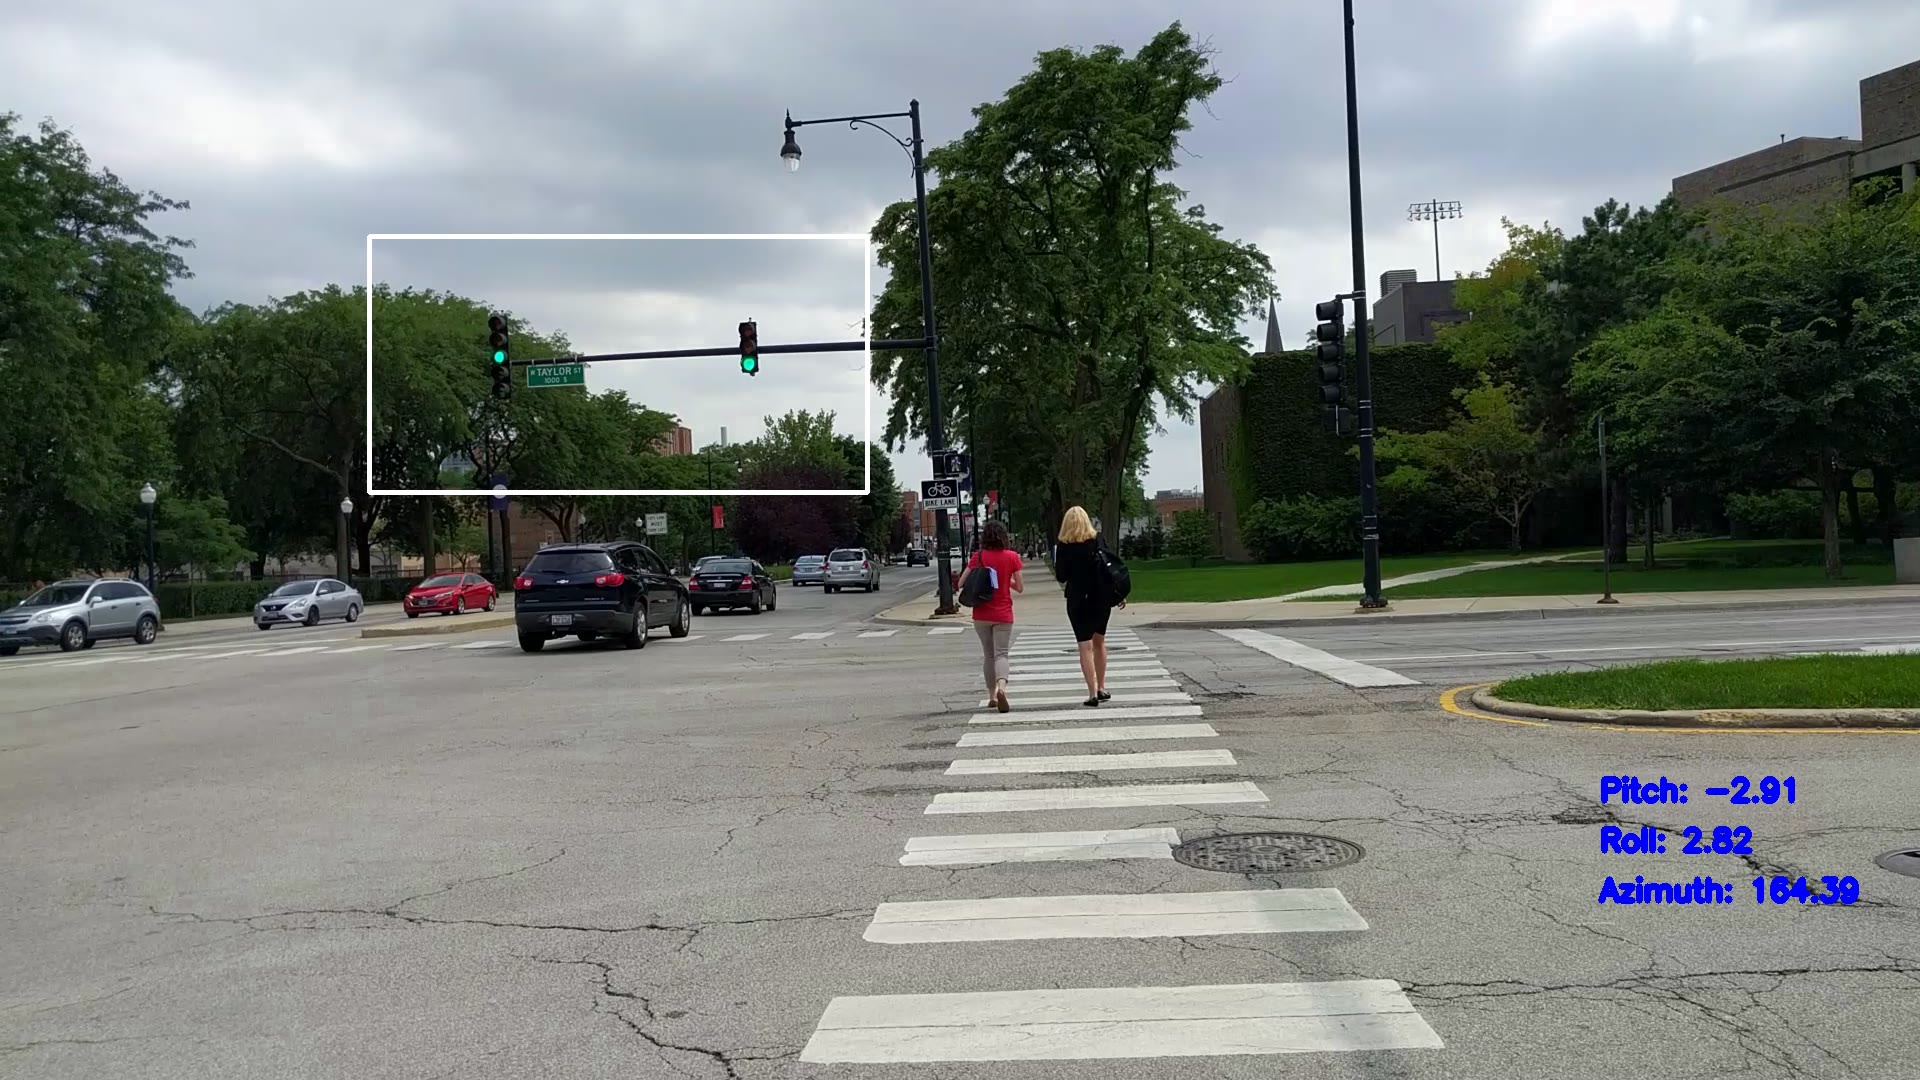
\includegraphics[width=4.2in]{images/rec_mv.jpg}}\\
\subfloat[Movement with change of sensor data] {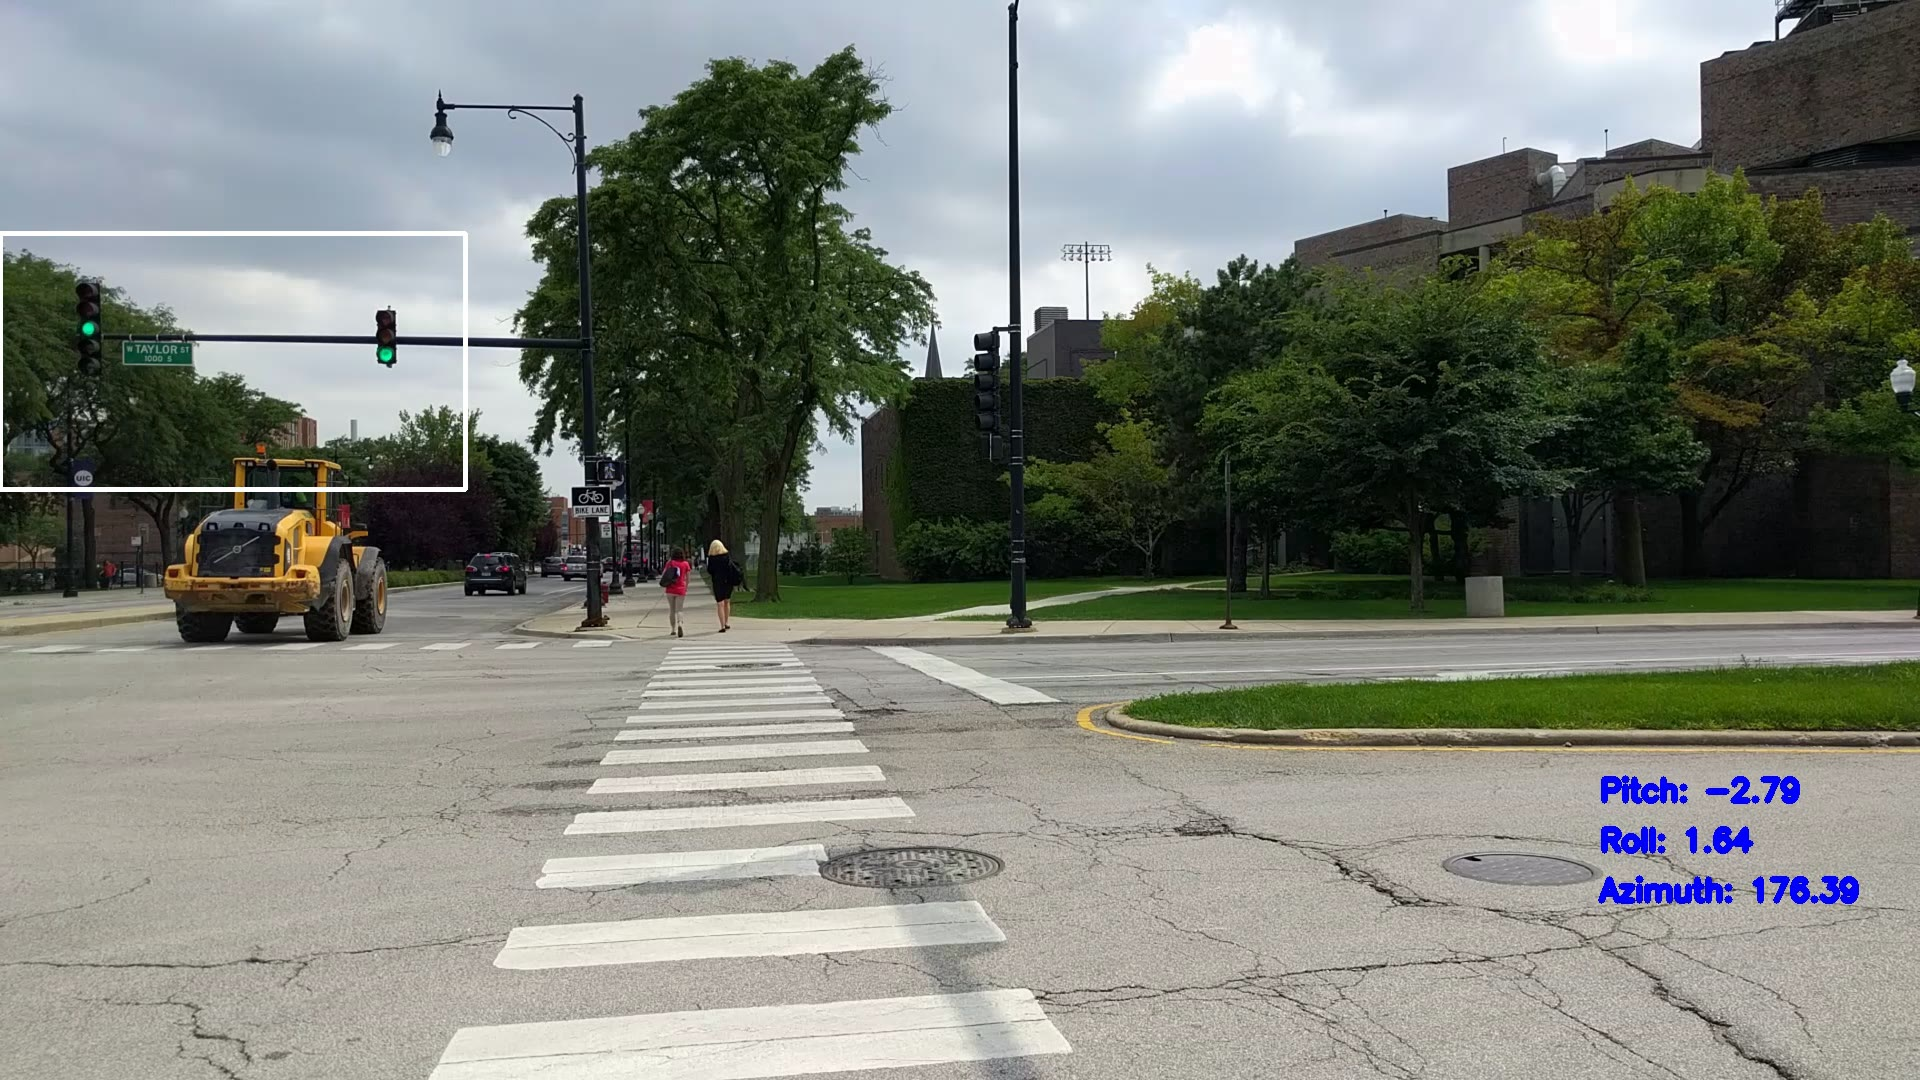
\includegraphics[width=4.2in]{images/rec_mv1.jpg}}\\
\subfloat[Movement with change of sensor data] {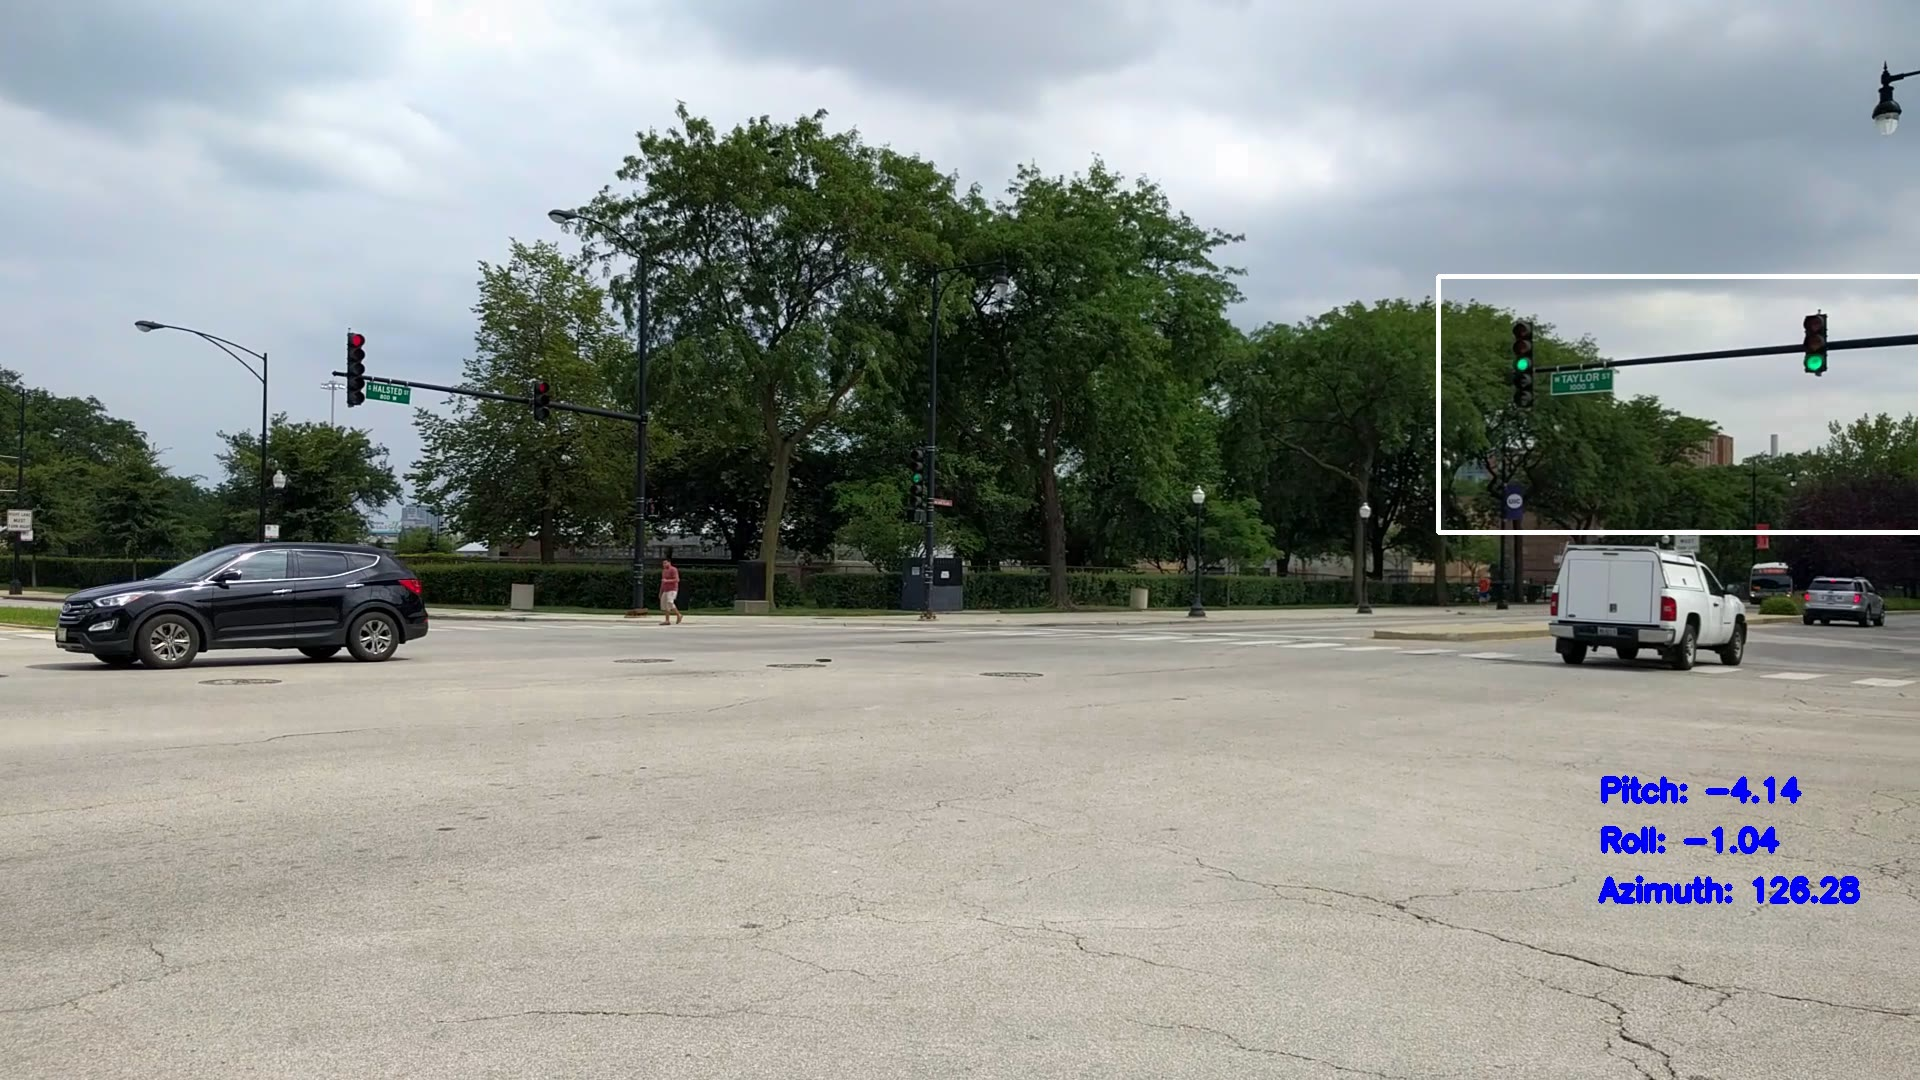
\includegraphics[width=4.2in]{images/rec_mv2.jpg}}
\caption{ROI movement with the change of sensor data.}
\label{f:rec_mv}
\end{figure*}

%Apart from this, when our system can not detect any circle in our specific ROI area, it updates the ROI and tries to detect the light.

%With the successful detection, our region of interest updates to new position with the light position and pitch and azimuth value.

However, when our prediction is inaccurate (discussed more at \ref{s:overview}), we gradually increase the ROI.
In this case, we already processed some part of the video frame. 
Hence, to avoid the double processing, we increase the region in the surrounding sides of the previous ROI having unsuccessful detection.
If at detect traffic lights in any of these areas, we reset the ROI to its original size in subsequent frames.
We illustrate this process with an example in \ref{f:rectangle}.
It shows that the rectangle A (original ROI) does not detect any traffic light.
Hence, we enlarge the ROI with 4 four rectangles named B, C, D, and E and traffic lights are detected in rectangle B.
Note that  we keep an overlap between the original ROI and new rectangles so that we do not miss any circles that fall in the boundary. 


\begin{figure}
\centering
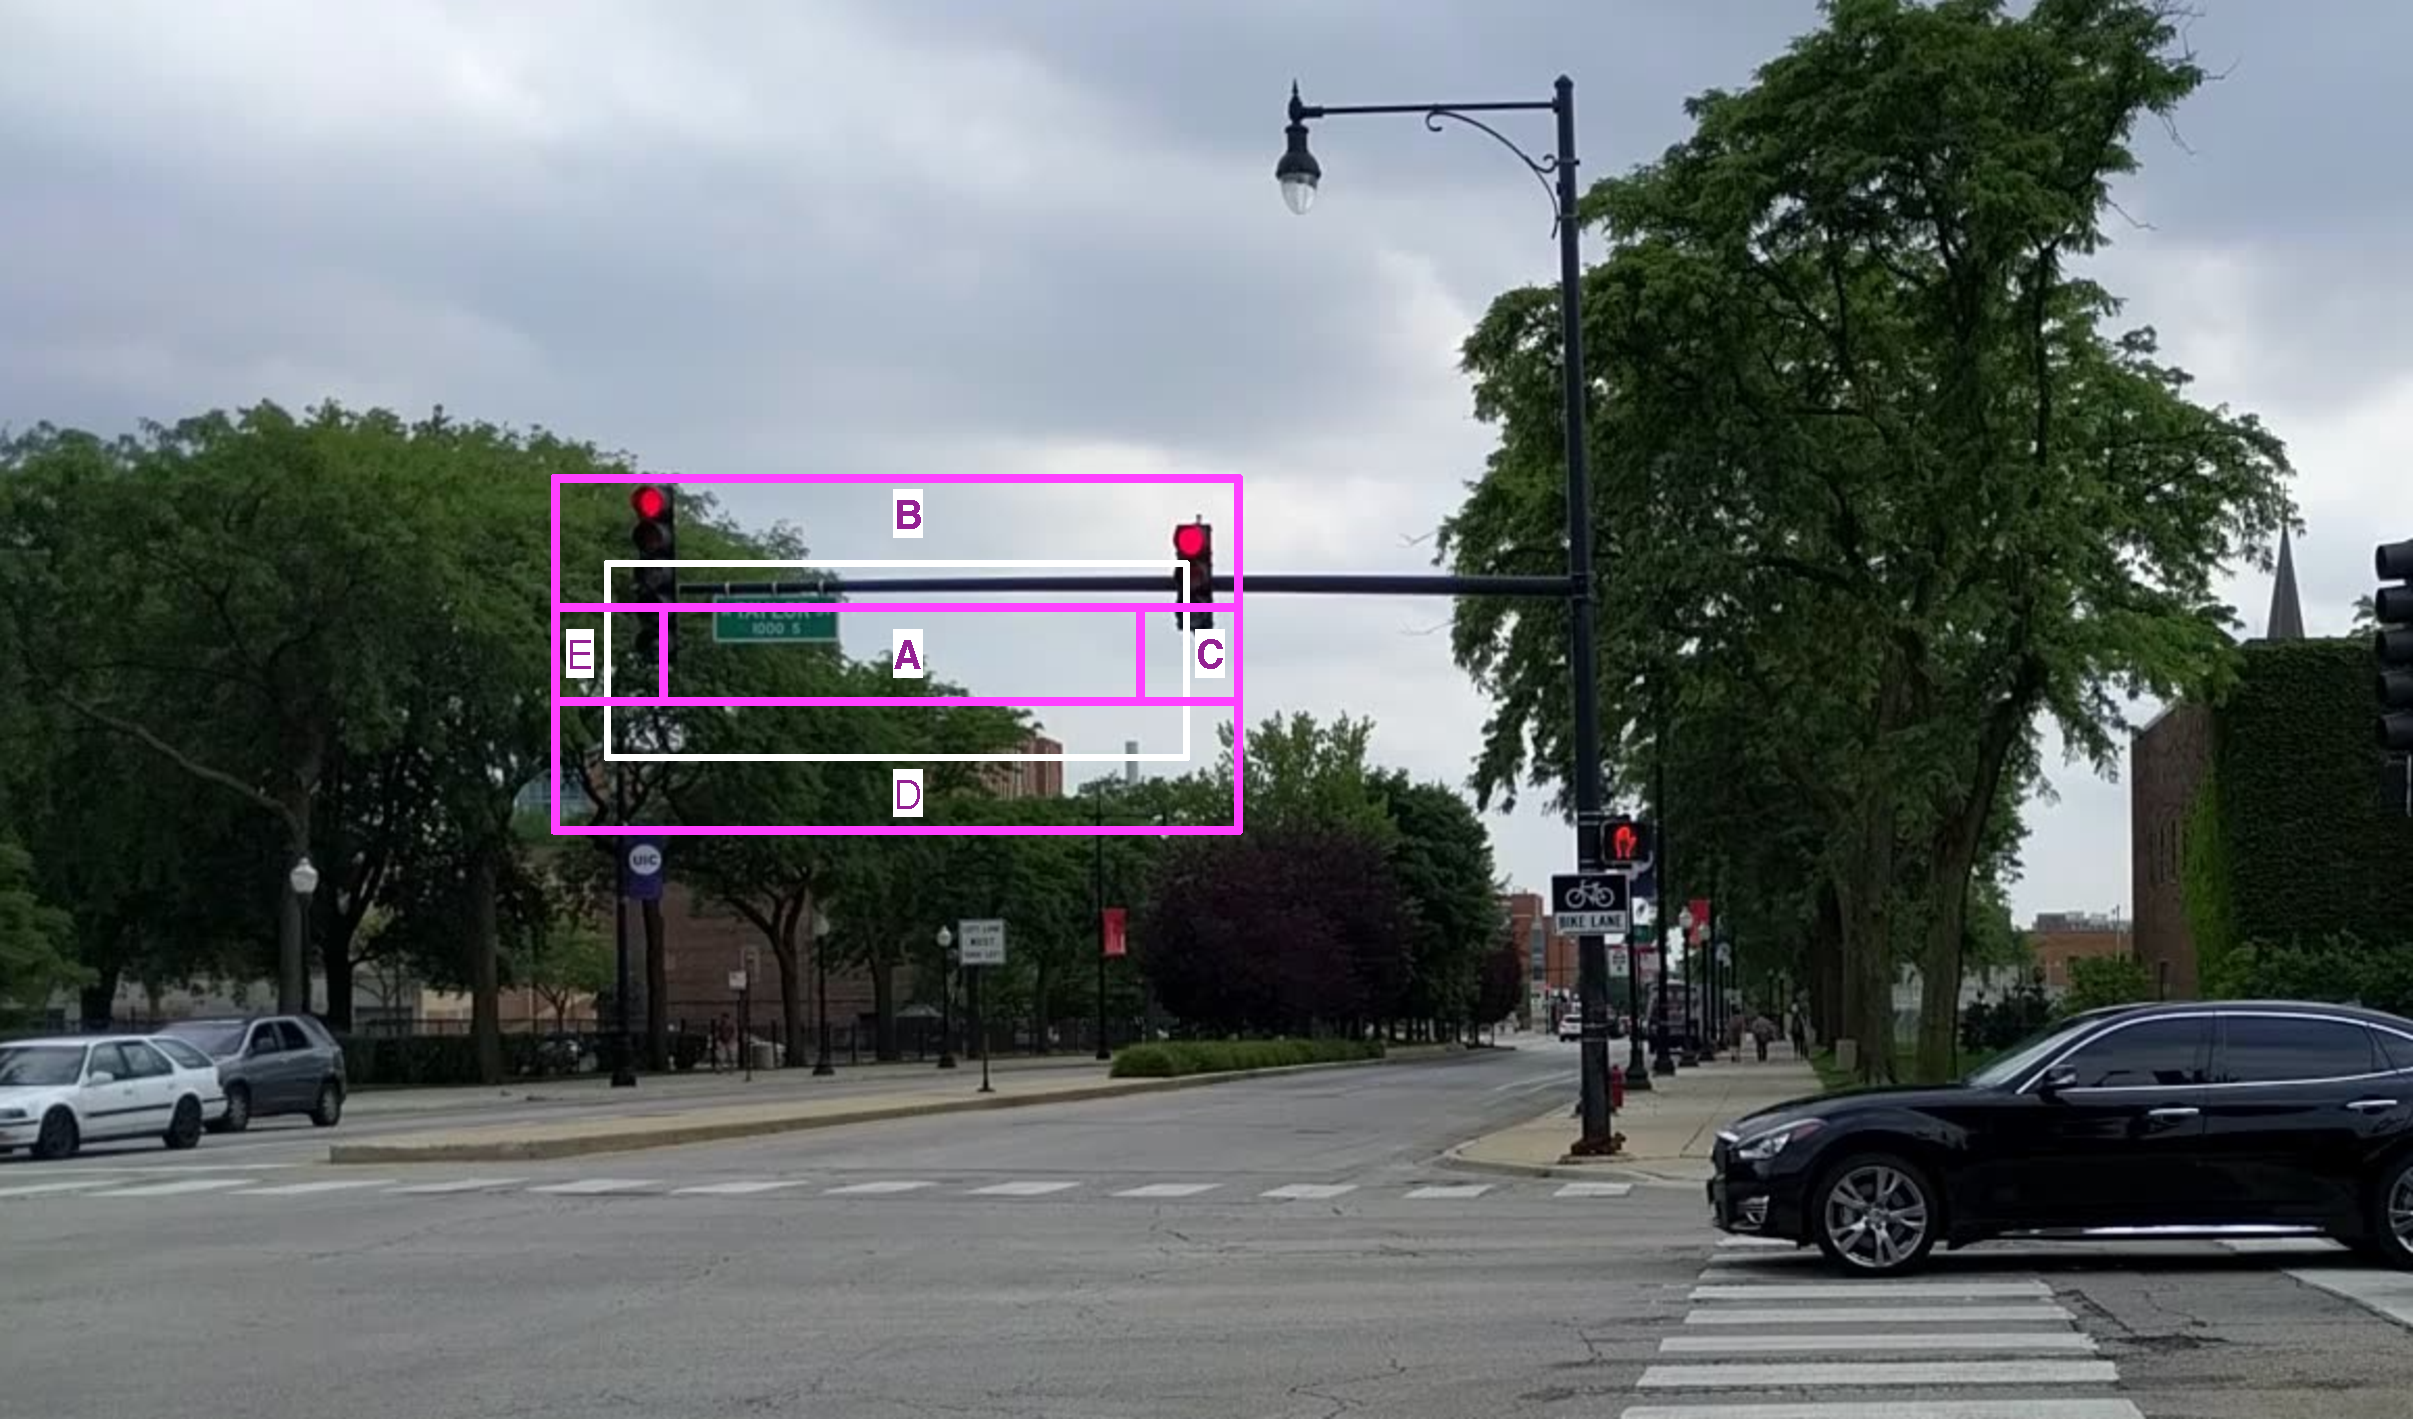
\includegraphics[width=5.2in]{figures/rectangle.pdf}
\caption{ROI increment policy}
\label{f:rectangle}
\end{figure}

\begin{figure*}[!ht]
\centering
\subfloat {\label{f:enl}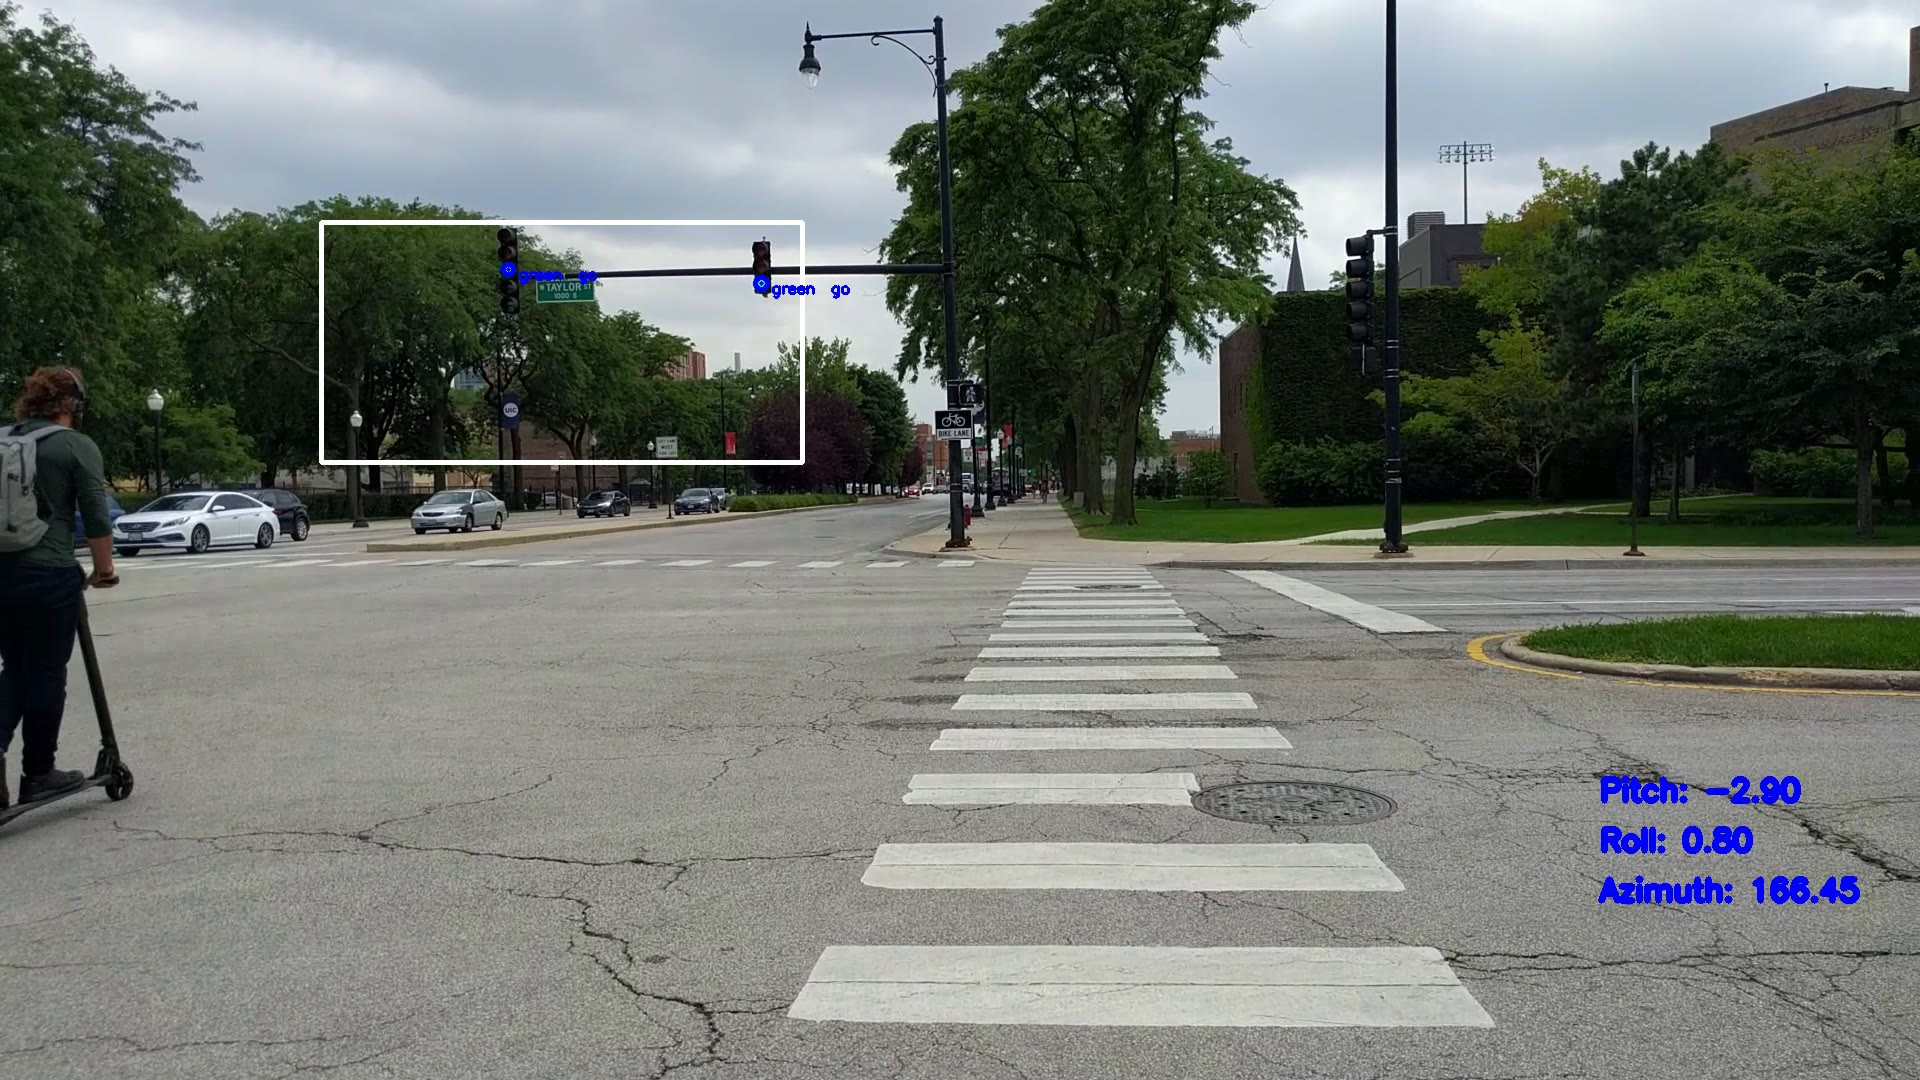
\includegraphics[width=4.2in]{images/rec_enl.jpg}}\\
\subfloat {\label{f:enl1}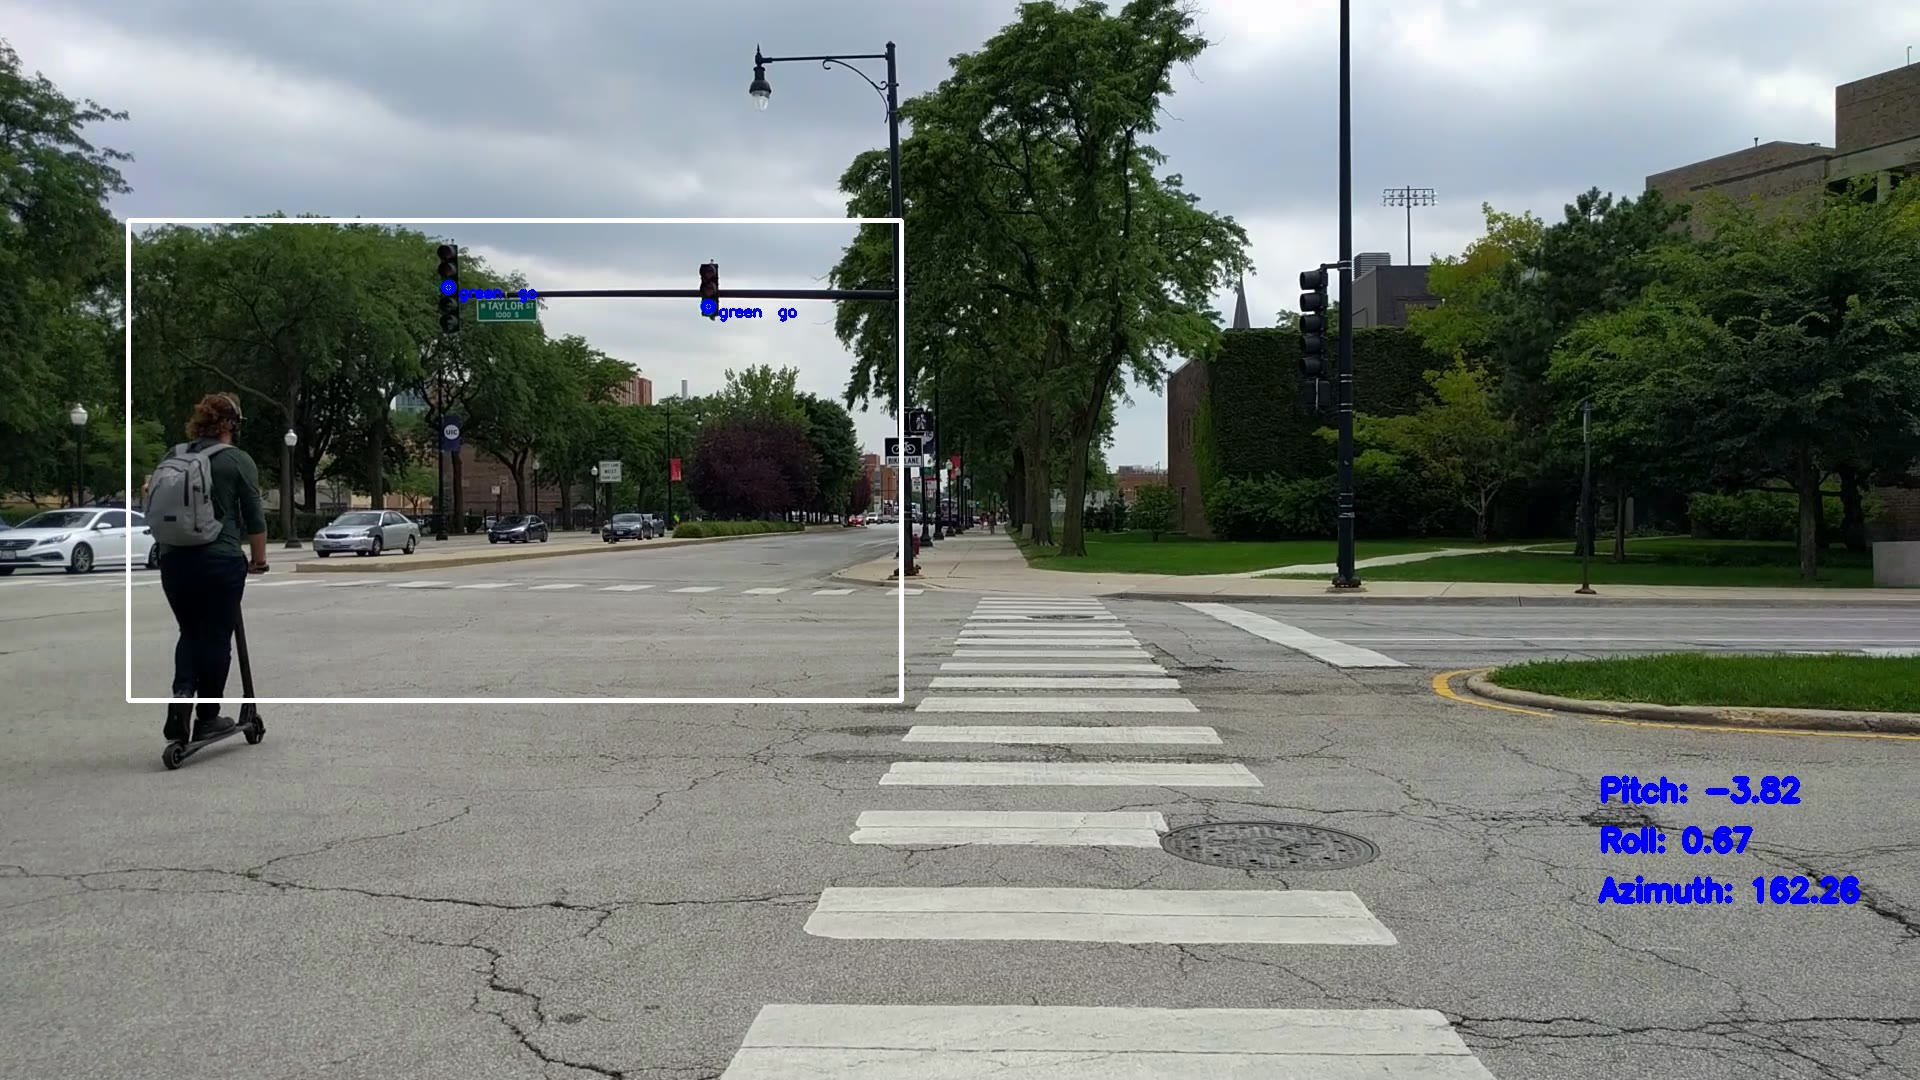
\includegraphics[width=4.2in]{images/rec_enl1.jpg}}
\caption{Enlarged ROI to detect traffic light successfully.}
\label{f:rec_enl}
\end{figure*}

\ref{f:rec_enl} shows the change of ROI to the subsequent frames.
Here, Figure \ref{f:enl} shows the video frame of a successful detection.
Figure \ref{f:enl1} shows the next frame, where detection goes wrong at first and we change the ROI in the next frame.



